% !TeX program = pdflatex
%DIF LATEXDIFF DIFFERENCE FILE
%DIF DEL /home/jovyan/FedLoRA_remote_package/2_latex及附属文件历史版本/CN_package_v4_backup/CN_reviewed_pre_polish.tex   Sun Sep 20 13:09:02 2026
%DIF ADD CN_reviewed.tex                                                                                                          Mon Sep 21 00:33:15 2026
\documentclass[preprint,12pt]{elsarticle}
\journal{Computer Networks}
\usepackage{amsmath,amssymb,amsthm,booktabs,graphicx,algorithm,algorithmic,multirow}
\usepackage{float}
\newtheorem{proposition}{Proposition}
\emergencystretch=1.5em
\usepackage{tikz}
\usetikzlibrary{arrows.meta,positioning,fit,calc}
%DIF PREAMBLE EXTENSION ADDED BY LATEXDIFF
%DIF UNDERLINE PREAMBLE %DIF PREAMBLE
\RequirePackage[normalem]{ulem} %DIF PREAMBLE
\RequirePackage{color}\definecolor{RED}{rgb}{1,0,0}\definecolor{BLUE}{rgb}{0,0,1} %DIF PREAMBLE
\providecommand{\DIFadd}[1]{{\protect\color{blue}\uwave{#1}}} %DIF PREAMBLE
\providecommand{\DIFdel}[1]{{\protect\color{red}\sout{#1}}}                      %DIF PREAMBLE
%DIF SAFE PREAMBLE %DIF PREAMBLE
\providecommand{\DIFaddbegin}{} %DIF PREAMBLE
\providecommand{\DIFaddend}{} %DIF PREAMBLE
\providecommand{\DIFdelbegin}{} %DIF PREAMBLE
\providecommand{\DIFdelend}{} %DIF PREAMBLE
\providecommand{\DIFmodbegin}{} %DIF PREAMBLE
\providecommand{\DIFmodend}{} %DIF PREAMBLE
%DIF FLOATSAFE PREAMBLE %DIF PREAMBLE
\providecommand{\DIFaddFL}[1]{\DIFadd{#1}} %DIF PREAMBLE
\providecommand{\DIFdelFL}[1]{\DIFdel{#1}} %DIF PREAMBLE
\providecommand{\DIFaddbeginFL}{} %DIF PREAMBLE
\providecommand{\DIFaddendFL}{} %DIF PREAMBLE
\providecommand{\DIFdelbeginFL}{} %DIF PREAMBLE
\providecommand{\DIFdelendFL}{} %DIF PREAMBLE
\newcommand{\DIFscaledelfig}{0.5}
%DIF HIGHLIGHTGRAPHICS PREAMBLE %DIF PREAMBLE
\RequirePackage{settobox} %DIF PREAMBLE
\RequirePackage{letltxmacro} %DIF PREAMBLE
\newsavebox{\DIFdelgraphicsbox} %DIF PREAMBLE
\newlength{\DIFdelgraphicswidth} %DIF PREAMBLE
\newlength{\DIFdelgraphicsheight} %DIF PREAMBLE
% store original definition of \includegraphics %DIF PREAMBLE
\LetLtxMacro{\DIFOincludegraphics}{\includegraphics} %DIF PREAMBLE
\newcommand{\DIFaddincludegraphics}[2][]{{\color{blue}\fbox{\DIFOincludegraphics[#1]{#2}}}} %DIF PREAMBLE
\newcommand{\DIFdelincludegraphics}[2][]{% %DIF PREAMBLE
\sbox{\DIFdelgraphicsbox}{\DIFOincludegraphics[#1]{#2}}% %DIF PREAMBLE
\settoboxwidth{\DIFdelgraphicswidth}{\DIFdelgraphicsbox} %DIF PREAMBLE
\settoboxtotalheight{\DIFdelgraphicsheight}{\DIFdelgraphicsbox} %DIF PREAMBLE
\scalebox{\DIFscaledelfig}{% %DIF PREAMBLE
\parbox[b]{\DIFdelgraphicswidth}{\usebox{\DIFdelgraphicsbox}\\[-\baselineskip] \rule{\DIFdelgraphicswidth}{0em}}\llap{\resizebox{\DIFdelgraphicswidth}{\DIFdelgraphicsheight}{% %DIF PREAMBLE
\setlength{\unitlength}{\DIFdelgraphicswidth}% %DIF PREAMBLE
\begin{picture}(1,1)% %DIF PREAMBLE
\thicklines\linethickness{2pt} %DIF PREAMBLE
{\color[rgb]{1,0,0}\put(0,0){\framebox(1,1){}}}% %DIF PREAMBLE
{\color[rgb]{1,0,0}\put(0,0){\line( 1,1){1}}}% %DIF PREAMBLE
{\color[rgb]{1,0,0}\put(0,1){\line(1,-1){1}}}% %DIF PREAMBLE
\end{picture}% %DIF PREAMBLE
}\hspace*{3pt}}} %DIF PREAMBLE
} %DIF PREAMBLE
\LetLtxMacro{\DIFOaddbegin}{\DIFaddbegin} %DIF PREAMBLE
\LetLtxMacro{\DIFOaddend}{\DIFaddend} %DIF PREAMBLE
\LetLtxMacro{\DIFOdelbegin}{\DIFdelbegin} %DIF PREAMBLE
\LetLtxMacro{\DIFOdelend}{\DIFdelend} %DIF PREAMBLE
\DeclareRobustCommand{\DIFaddbegin}{\DIFOaddbegin \let\includegraphics\DIFaddincludegraphics} %DIF PREAMBLE
\DeclareRobustCommand{\DIFaddend}{\DIFOaddend \let\includegraphics\DIFOincludegraphics} %DIF PREAMBLE
\DeclareRobustCommand{\DIFdelbegin}{\DIFOdelbegin \let\includegraphics\DIFdelincludegraphics} %DIF PREAMBLE
\DeclareRobustCommand{\DIFdelend}{\DIFOaddend \let\includegraphics\DIFOincludegraphics} %DIF PREAMBLE
\LetLtxMacro{\DIFOaddbeginFL}{\DIFaddbeginFL} %DIF PREAMBLE
\LetLtxMacro{\DIFOaddendFL}{\DIFaddendFL} %DIF PREAMBLE
\LetLtxMacro{\DIFOdelbeginFL}{\DIFdelbeginFL} %DIF PREAMBLE
\LetLtxMacro{\DIFOdelendFL}{\DIFdelendFL} %DIF PREAMBLE
\DeclareRobustCommand{\DIFaddbeginFL}{\DIFOaddbeginFL \let\includegraphics\DIFaddincludegraphics} %DIF PREAMBLE
\DeclareRobustCommand{\DIFaddendFL}{\DIFOaddendFL \let\includegraphics\DIFOincludegraphics} %DIF PREAMBLE
\DeclareRobustCommand{\DIFdelbeginFL}{\DIFOdelbeginFL \let\includegraphics\DIFdelincludegraphics} %DIF PREAMBLE
\DeclareRobustCommand{\DIFdelendFL}{\DIFOaddendFL \let\includegraphics\DIFOincludegraphics} %DIF PREAMBLE
%DIF COLORLISTINGS PREAMBLE %DIF PREAMBLE
\RequirePackage{listings} %DIF PREAMBLE
\RequirePackage{color} %DIF PREAMBLE
\lstdefinelanguage{DIFcode}{ %DIF PREAMBLE
%DIF DIFCODE_UNDERLINE %DIF PREAMBLE
  moredelim=[il][\color{red}\sout]{\%DIF\ <\ }, %DIF PREAMBLE
  moredelim=[il][\color{blue}\uwave]{\%DIF\ >\ } %DIF PREAMBLE
} %DIF PREAMBLE
\lstdefinestyle{DIFverbatimstyle}{ %DIF PREAMBLE
	language=DIFcode, %DIF PREAMBLE
	basicstyle=\ttfamily, %DIF PREAMBLE
	columns=fullflexible, %DIF PREAMBLE
	keepspaces=true %DIF PREAMBLE
} %DIF PREAMBLE
\lstnewenvironment{DIFverbatim}{\lstset{style=DIFverbatimstyle}}{} %DIF PREAMBLE
\lstnewenvironment{DIFverbatim*}{\lstset{style=DIFverbatimstyle,showspaces=true}}{} %DIF PREAMBLE
%DIF END PREAMBLE EXTENSION ADDED BY LATEXDIFF

\begin{document}
\begin{frontmatter}
\title{FedRAS: Network-Conditioned Rank Allocation for Federated LoRA}
\author[inst1,inst2,inst3]{Wenyu Ma}
\author[inst1,inst2,inst3]{Tao Hu\corref{cor1}}
\ead{hutaondsc@163.com}
\author[inst1,inst2,inst3]{Xinlei Liu}
\cortext[cor1]{Corresponding author}
\address[inst1]{Information Engineering University, Zhengzhou 450001, China}
\address[inst2]{Key Laboratory of Cyberspace Endogenous Safety and Security of Henan Province, Zhengzhou 450001, China}
\address[inst3]{Key Laboratory of Cyberspace Security, Ministry of Education of China, Zhengzhou 450001, China}

\begin{abstract}
Federated LoRA reduces update size, but a fixed rank cannot adapt to time-varying links. We formulate rank selection and client admission as a joint network scheduling problem and call the resulting method FedRAS. It estimates a delivery probability and an adaptation capacity for each client--rank pair, maximizes the expected useful updates under byte-budget and participation constraints, solves the assignment with a dynamic program, and aggregates heterogeneous ranks with frozen-factor rank masking. All payloads are accounted at their real serialized sizes: a frozen-$A$ client uploads only the trainable $B$ factor, 0.090\,MB per round at rank 16, against 5.29\,MB for a full-model update.

Experiments on non-IID CIFAR-10, CIFAR-100, and MNIST with a 500-client scheduler simulation use deadlines recalibrated to these real payloads. At the nominal deadline, rank selection reduces to fixed rank-16 behavior at zero cost. Under a 0.1\,s deadline, FedRAS delivers 22\% more timely updates and 23\% fewer bytes than fixed rank 16 over ten seeds ($p{=}0.002$), while a full-model update misses every \DIFaddbegin \DIFadd{stress }\DIFaddend deadline and spends $58.7\times$ the bytes. A pre-registered TOST equivalence test confirms that accuracy is preserved. The dynamic program improves on greedy scheduling by \DIFaddbegin \DIFadd{28 to 55\% when the budget binds, and by }\DIFaddend up to 64\% \DIFdelbegin \DIFdel{in binding regimes at 23--836}\DIFdelend \DIFaddbegin \DIFadd{over value-per-byte pricing, at 23--421}\DIFaddend \,ms solver cost, and a deliberately miscalibrated delivery predictor costs at most 1\% of the assignment objective. These results describe network-side gains in the evaluated frozen-backbone setting and do not imply universal accuracy gains.
\end{abstract}

\begin{keyword}
Federated LoRA \sep Mobile edge computing \sep Rank selection \sep Deadline scheduling \sep Wireless federated learning
\end{keyword}
\end{frontmatter}

\section{Introduction}
\label{sec:intro}

Mobile edge networks increasingly host federated learning (FL) workloads in which heterogeneous clients such as smartphones, vehicles, UAV terminals, and satellite-connected devices collaborate on a shared model without exposing raw data \cite{mcmahan2017fedavg,kairouz2021advances,liu2018sagin,mahboob2024ntn}. The dominant cost in such systems is the uplink. Full-parameter model updates saturate wireless capacity, drain client energy, and frequently miss round deadlines when links degrade during handover or outage, as reported for ground, aerial, and satellite segments \cite{razmi2022ground,tang2023flsagin,qin2024dfrl,ribero2023intermittent}. Low-rank adaptation (LoRA) has therefore become an attractive transmission format for FL, because only two small factor matrices per adapted layer are communicated instead of the full weight delta \cite{hu2022lora,babakniya2023slora,zhang2024fedit}.

Existing Federated LoRA systems, however, treat the rank $r$ as a model hyperparameter. The rank is selected from data and system constraints alone, possibly varying across clients \cite{cho2024hetlora,fan2025helora} or adapting across rounds \cite{wu2026fedara,yang2024safedlora}, but not from the state of a lossy, deadline-constrained link. This convention ignores a scheduling dimension that is directly visible to the network. \DIFaddbegin \DIFadd{The omitted coupling is mechanical. A larger rank transmits more bytes and therefore loses delivery probability exactly where it gains adaptation capacity, while a smaller rank travels light but forfeits capacity on the healthy links that could have carried it. Whether the extra capacity is worth the delivery risk depends on the link state, and no training-side rule observes that state.
}\DIFaddend 

This raises three questions. How should delivery probability depend on rank and observable link state? How should client--rank assignment be solved under budget and participation constraints? Does the resulting adaptation improve network behavior in a real trainer? \DIFaddbegin \DIFadd{These questions are answered in Sections~\ref{sec:model}, \ref{sec:solver}, and \ref{sec:eval}, respectively.
}\DIFaddend 

\subsection{Contributions}
We answer these questions with a delivery model, a grid-based dynamic-programming solver, a rank-selection rule, and a two-tier evaluation. We call the method FedRAS. The contributions are as follows.

\begin{itemize}
\item \textbf{Deadline-aware client--rank model.} We formulate each round as a joint assignment in which admission and rank are selected together. The model links rank to its real serialized payload, a delivery probability $P_{\mathrm{on}}(r)$, and a saturating capacity gain $G(r)$. Sections~\ref{sec:model} and \ref{sec:problem} develop the model.
\item \textbf{Dynamic-programming scheduler.} The estimated problem is a multiple-choice knapsack with an admission cap. We derive a pseudo-polynomial dynamic program that is exact for the discretized single-round estimated assignment problem, with complexity $O(|\mathcal D| K B_{\max}|\mathcal R|)$. The solver study measures greedy gaps and runtime.
\item \textbf{Heterogeneous-rank aggregation.} We use rank-masked averaging with a shared frozen $A$ factor, so only the trainable $B$ factor is ever uploaded. Under this condition, the rule gives exact coordinate-wise averaging of active induced-update slices. Proposition~\ref{prop:agg} states the conditions and limits.
\item \textbf{Two-tier evaluation at real payload sizes.} A real trainer covers non-IID CIFAR-10, CIFAR-100, and MNIST over ten seeds, and a 500-client scheduler simulation covers deadline, budget, mobility, and scale regimes. Under a 0.1\,s deadline, FedRAS delivers 22\% more timely updates and 23\% fewer bytes than fixed rank 16 at equivalent accuracy, while full-parameter updates miss every \DIFaddbegin \DIFadd{stress }\DIFaddend deadline at $58.7\times$ the bytes. The evaluation further covers external baselines, a candidate-pool decomposition of the scheduler's gains, a SAGIN link profile, and pre-registered equivalence tests.
\end{itemize}

A preliminary poster version of this work studied joint client--protection scheduling for federated learning in space--air--ground mobile networks \cite{ma2026mswim}. The present article substantially reformulates that line of work around a different schedulable resource. It replaces compression-and-protection policies with the LoRA rank as the per-client decision variable. It introduces the real-payload delivery hazard and the saturating capacity model of Section~\ref{sec:model}, replaces the heuristic admission-and-repair procedure with a dynamic program that is exact on the stated budget grid, and adds frozen-factor rank-masked aggregation for heterogeneous ranks. It also reports a new two-tier evaluation comprising a real federated LoRA trainer, a 500-client scheduling simulator, and a solver exactness study. Accordingly, all numerical results in this article come from the revised formulation and implementation and are not comparable with the preliminary version.

We report accuracy, timely delivery ratio, and bytes per round separately. With a frozen pretrained backbone, the expected benefit of rank selection \DIFdelbegin \DIFdel{is }\DIFdelend \DIFaddbegin \DIFadd{lies }\DIFaddend on the network side rather than \DIFaddbegin \DIFadd{in }\DIFaddend universal accuracy improvement.

The remainder of this paper is organized as follows. Section~\ref{sec:related} reviews related work. Section~\ref{sec:model} introduces the system model. Section~\ref{sec:problem} formulates the scheduling problem and Section~\ref{sec:solver} presents the solver and the aggregation scheme. Section~\ref{sec:eval} reports the evaluation, Section~\ref{sec:discussion} discusses limitations, and Section~\ref{sec:conclusion} concludes.

\section{Related work}
\label{sec:related}

\subsection{Parameter-efficient and federated LoRA}
LoRA freezes a pretrained backbone and learns low-rank increments $\Delta W=BA$ \cite{hu2022lora}. Federated LoRA trains these adapters across clients. Prior work has studied sparse updates, instruction tuning, and model-heterogeneous personalization \cite{babakniya2023slora,zhang2024fedit,yi2026pfedlora}. A further line lets the rank vary across clients and aligns \DIFdelbegin \DIFdel{the results }\DIFdelend \DIFaddbegin \DIFadd{heterogeneous ranks }\DIFaddend for aggregation, by rank self-pruning with sparsity-weighted averaging \cite{cho2024hetlora}, stacking \cite{wang2024flora}, zero-padded rank alignment \cite{fan2025helora}, or SVD-based dynamic rank allocation \cite{wu2026fedara}.

FFA-LoRA \cite{sun2024ffalora} froze one factor at its random initialization and showed that this improves stability in privacy-preserving federated fine-tuning. We adopt the same frozen-factor property for a stronger reason. When the frozen factor is identical across clients, averaging the trainable factor gives exact coordinate-wise averaging of the active induced-update slices, as Proposition~\ref{prop:agg} shows, and each client uploads only that factor. It thereby removes the factor-rotation ambiguity that makes joint factor averaging differ from update averaging. Section~\ref{sec:aggregation} develops this aggregation.

SA-FedLoRA schedules rank over rounds without conditioning on link state \cite{yang2024safedlora}. FedSA-LoRA studies asymmetric factor aggregation with client-local parameters \cite{guo2025fedsalora}. These rank-adaptation rules respond to training progress or device capability, not to the delivery state of a deadline-constrained link. We evaluate an annealing baseline and joint A/B averaging while making rank a per-round decision conditioned on delivery state and deadline.

\subsection{Communication-efficient federated learning}
A broad literature reduces FL communication through sparsification, quantization, compressed sensing, and over-the-air aggregation \cite{oh2023fedqcs,oh2024fedvqcs,liu2023adaptivequant,kim2023beamforming,reisizadeh2020fedpaq,lin2018deep}. These methods compress a given update. Our scheduler selects its rank before transmission, so rank directly affects payload and deadline feasibility. The proposed capacity and delivery models can therefore be combined with other codecs.

\subsection{Client selection and deadline-aware scheduling}
Client selection improves FL efficiency under data, latency, and energy heterogeneity \cite{oort2021oort,chen2024clientselection,dong2024aoi,luo2021costeffective}. Deadline- and reliability-aware participation has also been studied in mobile and non-terrestrial networks \cite{razmi2022ground,tang2023flsagin,qin2024dfrl,ribero2023intermittent,han2024orchestrating}, and FedSN coordinates federated training across heterogeneous LEO satellite networks \cite{lin2025fedsn}. These methods generally treat update size as fixed. We include an Oort-style selector as a selection baseline. FedRAS chooses participation and update rank together, yielding a multiple-choice knapsack.

\subsection{Positioning}
We do not claim each ingredient individually as new. Our contribution is their combination. It comprises the LoRA rank treated as a deadline-constrained network resource with an explicit payload-conditioned delivery hazard, a client--rank assignment that is exact on the stated budget grid, with quantified greedy gaps and solver cost, and validation of the resulting trade-offs with a real federated trainer in which adapters are placed on every block of the backbone and all byte accounting uses real serialized sizes. The \DIFaddbegin \DIFadd{theoretical contribution is mechanism correctness rather than a learning-performance guarantee: exactness of the assignment on the stated grid (Proposition~\ref{prop:dp}) and exactness of frozen-factor aggregation (Proposition~\ref{prop:agg}), each with its scope conditions stated where it applies. The }\DIFaddend claim is conditional on the surveyed literature of Section~\ref{sec:related} and on the evaluated setting.

\section{System model}
\label{sec:model}

\begin{figure}[t]
\centering
\resizebox{\columnwidth}{!}{%
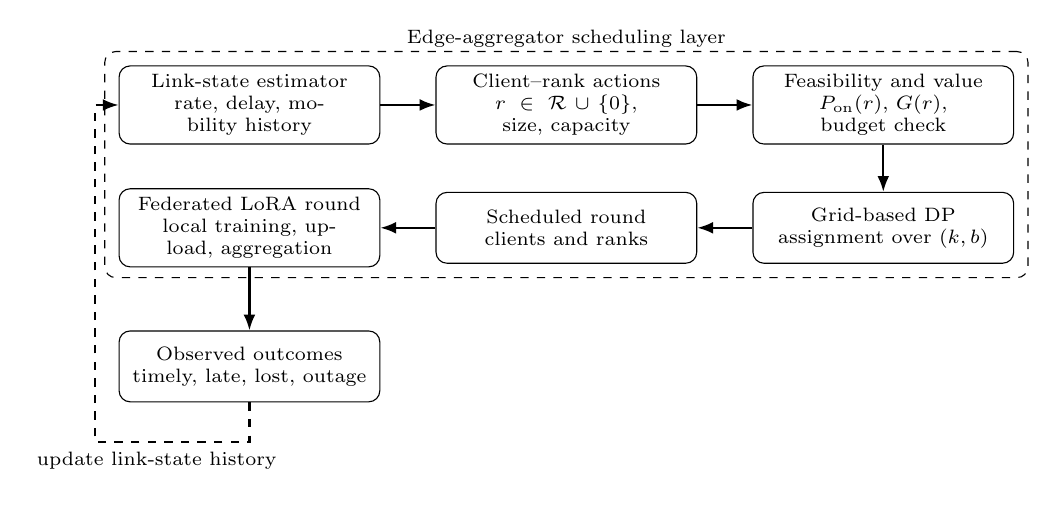
\begin{tikzpicture}[
  node distance=6mm and 7mm, >=Latex,
  box/.style={draw, rounded corners, align=center, minimum height=9mm, text width=31mm, font=\scriptsize, inner sep=3pt},
  flow/.style={-{Latex[length=2mm]}, thick},
  feedback/.style={-{Latex[length=2mm]}, dashed, thick}
]
\node[box] (estimate) {Link-state estimator\\rate, delay, mobility history};
\node[box, right=of estimate] (actions) {Client--rank actions\\$r\in\mathcal R\cup\{0\}$, size, capacity};
\node[box, right=of actions] (filter) {Feasibility and value\\$P_{\rm on}(r)$, $G(r)$, budget check};
\node[box, below=of filter] (dp) {Grid-based DP\\assignment over $(k,b)$};
\node[box, left=of dp] (assign) {Scheduled round\\clients and ranks};
\node[box, left=of assign] (fl) {Federated LoRA round\\local training, upload, aggregation};
\node[box, below=8mm of fl] (observe) {Observed outcomes\\timely, late, lost, outage};
\draw[flow] (estimate) -- (actions);
\draw[flow] (actions) -- (filter);
\draw[flow] (filter) -- (dp);
\draw[flow] (dp) -- (assign);
\draw[flow] (assign) -- (fl);
\draw[flow] (fl) -- (observe);
\coordinate (fb) at ($(fl.south)+(0,-4mm)$);
\draw[feedback] (observe.south) -- ++(0,-5mm) -| node[below, font=\scriptsize, pos=.3] {update link-state history} ($(estimate.west)+(-3mm,0)$) -- (estimate.west);
\node[draw, dashed, rounded corners, fit=(estimate)(actions)(filter)(dp)(assign), inner sep=5pt,
      label={[fill=white, inner sep=1pt, font=\scriptsize]above:Edge-aggregator scheduling layer}] {};
\end{tikzpicture}%
}
\caption{Round pipeline of FedRAS. The edge aggregator jointly selects clients and LoRA ranks with the grid-based dynamic program; only observed transmission outcomes update the link-state history.}
\label{fig:architecture}
\end{figure}

\subsection{Mobile edge FL architecture}
We consider a mobile edge network in which an edge aggregator serves a client set
$\mathcal{D}=\mathcal{D}_g\cup\mathcal{D}_a\cup\mathcal{D}_s$ of ground clients $\mathcal{D}_g$, aerial and UAV clients $\mathcal{D}_a$, and satellite-connected clients $\mathcal{D}_s$. Ground links are comparatively stable, aerial links face frequent handover, and satellite links suffer long propagation delay, intermittent visibility, and outages \cite{mahboob2024ntn,razmi2022ground}. The aggregator holds the global model, schedules every round, and aggregates the timely updates. Fig.~\ref{fig:architecture} shows the resulting round pipeline. In every round the aggregator estimates the link states, constructs and filters the client--rank actions, and solves the assignment with the grid-based dynamic program of Section~\ref{sec:solver}. It then executes the federated round and feeds the observed delivery outcomes back into the link-state history. The experiments evaluate both a homogeneous link profile and a grouped ground--aerial--satellite profile with distinct rate and mobility laws (Section~\ref{sec:eval}).

\subsection{Federated LoRA rounds}
Let $w^t$ denote the frozen backbone broadcast at round $t$. Client $i$ trains LoRA factors $A_{i,\ell}$ and $B_{i,\ell}$ for the adapted layers $\ell\in\mathcal L$. The effective weight change is $\Delta W_{i,\ell}=B_{i,\ell}A_{i,\ell}$. A rank $r$ update uses the first $r$ columns of $B_{i,\ell}$ and the matching rows of the shared $A$. A round then proceeds as follows. The aggregator broadcasts the backbone and the current adapter state. It observes the client link states and solves the client--rank assignment under the deadline, budget, and participation constraints. The admitted clients train locally with their factors truncated to the assigned rank, so only the first $r$ coordinates \DIFdelbegin \DIFdel{are ever trained}\DIFdelend \DIFaddbegin \DIFadd{receive gradient updates}\DIFaddend , and upload before the deadline $\tau$. The aggregator aggregates the timely updates with data-size weights and updates its link-state history from the observed outcomes. Late or lost updates are discarded, because stale updates harm convergence stability in deadline-critical federated learning.

\subsection{Link, mobility, and delivery model}
At decision time the scheduler receives an estimated uplink rate $\bar R_i^t$ in Mbps and a mobility state. The realized rate $R_i^t$, handover event $H_i^t\in\{0,1\}$, and packet loss indicator $J_i^t$ are not observed before transmission. For an update of $B_i^t(r)$ megabytes, the modeled delivery time is
\begin{equation}
T_i^t(r)=T_{\rm train,i}(r)+T_{\rm proc,i}(r)+\frac{8B_i^t(r)}{R_i^t}+d_i^t+H_i^t\Delta d_h.
\label{eq:delivery}
\end{equation}
Timely delivery is the event
\begin{equation}
P_{\rm on,i}^t(r)=\Pr\!\left(T_i^t(r)\le\tau,\;J_i^t=0\mid x_i^t\right).
\label{eq:pon}
\end{equation}

The implementation uses the following hazard surrogate rather than a derived distribution for all terms in \eqref{eq:delivery}.
\begin{equation}
\hat P_{\rm on,i}^t(r)=\exp\!\big(-\mu_i^t\big)\exp\!\Big(-\frac{8B_i^t(r)}{\bar R_i^t\tau}\Big).
\label{eq:hazard}
\end{equation}
The dimensionless intensity $\mu_i^t$ summarizes \DIFdelbegin \DIFdel{mobility related }\DIFdelend \DIFaddbegin \DIFadd{mobility-related }\DIFaddend failure risk, packet loss, handover effects, and unmodeled processing time. It is not estimated by an EWMA in the present implementation. The experiments generate mobility state from the stated Beta model and provide that state and the generated rate as oracle estimates. Thus, \eqref{eq:hazard} is an idealized plug-in predictor used to isolate scheduling behavior. The calibration and noise studies assess sensitivity to this predictor, but they do not constitute calibration on measured wireless traces. Training and processing times are included in the conceptual delivery model but are not separately measured in the current experiments.

\subsection{Rank-dependent update size and capacity}
With $b$ bits per parameter and the frozen factor $A$ shared and never transmitted, a rank-$r$ client uploads only the trainable factor $B$, whose per-rank cost is the summed output dimension $D=\sum_{\ell\in\mathcal L}d_\ell$ of the adapted layers. The real serialized payload is
\begin{equation}
B_i^t(r)=\frac{b}{8}\,r\,D+B_{\rm meta},
\label{eq:size}
\end{equation}
in bytes, with $D=1{,}408$ parameters per rank column and $b=32$ in the evaluated CNN, giving $B^t(16)=0.090$\,MB \DIFdelbegin \DIFdel{including headers}\DIFdelend \DIFaddbegin \DIFadd{when the header allowance $B_{\rm meta}$ is set to zero in the metering (Table~\ref{tab:audit})}\DIFaddend . Rank is therefore a network-visible resource. It scales both the adaptation capacity and the transmission time. We model the useful contribution of a delivered rank-$r$ update with the saturating capacity gain
\begin{equation}
G_i^t(r)=\pi_i^t\,\sqrt{\min(r,r_{\max})/r_{\max}},
\label{eq:cap}
\end{equation}
where $\pi_i^t$ is a per-client contribution prior in the spirit of Oort-style utility \cite{oort2021oort}. The width $r_{\max}$ is the factor width provisioned at all clients. The square root encodes diminishing returns of rank; the trainer data support this shape, with the mean delivered update norm growing by \DIFdelbegin \DIFdel{$1.86\times$ }\DIFdelend \DIFaddbegin \DIFadd{about $1.9\times$ }\DIFaddend from rank 4 to rank 16 against the $4\times$ of a linear model. The saturation at $r_{\max}$ reflects that wider factors add payload but no expressible capacity once the provisioned width is reached. Full-parameter FedAvg updates are accounted at their true serialized size, $5.29$\,MB in the evaluated model, i.e., $58.7\times$ a rank-16 upload.

\section{Deadline-aware client--rank scheduling}
\label{sec:problem}

Each round, the aggregator decides $a_i^t\in\{0\}\cup\mathcal R$, where $a_i^t=0$ means client $i$ does not participate and $a_i^t=r$ schedules it at rank $r$. The per-round problem is
\begin{equation}
\max_{\{a_i^t\}}\;\sum_{i\in\mathcal D}\mathbf 1\{a_i^t>0\}\,G_i^t(a_i^t)\,P_{\rm on,i}^t(a_i^t)
\label{eq:objective}
\end{equation}
\begin{equation}
\text{s.t.}\quad \sum_i B_i^t(a_i^t)\le B_{\max},\qquad \sum_i\mathbf 1\{a_i^t>0\}\le K .
\label{eq:constraints}
\end{equation}
The objective is a scheduling utility. It counts expected useful delivered updates under the byte budget $B_{\max}$ and participation cap $K$. It is not a direct surrogate for final test accuracy. Increasing $r$ raises $G$ sublinearly, increases payload, and lowers the delivery surrogate. The experiments therefore report test accuracy, timely delivery ratio, bytes per round, and mean delivered rank as separate outcomes.

Two deployment variants are evaluated. In full grid scheduling, the aggregator solves \eqref{eq:objective} and \eqref{eq:constraints} over all clients. The solver study evaluates this variant at 500-client scale, and a same-cohort variant restricts the dynamic program to a uniformly sampled cohort, isolating the value of candidate-pool widening from in-cohort rank allocation. In the real trainer, fair-cohort scheduling samples the fixed cohort of ten clients and applies the per-client rank rule $r_i^\star=\arg\max_r G_i^t(r)P_{\rm on,i}^t(r)$. All budget arithmetic uses a conservative ceiling discretization onto a $0.01$\,MB grid, applied identically to the dynamic program, the greedy baselines, and the \DIFdelbegin \DIFdel{byte accounting}\DIFdelend \DIFaddbegin \DIFadd{admission checks}\DIFaddend , so that every \DIFaddbegin \DIFadd{scheduling }\DIFaddend method optimizes over the identical feasible region. Section~\ref{sec:dpvfair} compares the variants in the trainer.

\section{Grid-based solver and heterogeneous-rank aggregation}
\label{sec:solver}

\subsection{Dynamic program}
Problem \eqref{eq:objective}--\eqref{eq:constraints} is a multiple-choice knapsack with an admission constraint. Let $q=0.01$ MB be the budget grid and define the integer cost $\widetilde B_i(r)=\lceil B_i^t(r)/q\rceil$. Let $V_i(k,b)$ be the maximum estimated utility from the first $i$ clients with $k$ admissions and integer budget $b$. Initialize $V_0(0,0)=0$ and all other states to $-\infty$. The recurrence is
\begin{equation}
V_i(k,b)=\max\Big\{V_{i-1}(k,b),\;\max_{r\in\mathcal R}\big[V_{i-1}(k-1,b-\widetilde B_i(r))+u_i(r)\big]\Big\},
\label{eq:dp}
\end{equation}
where $u_i(r)=G_i^t(r)\hat P_{\rm on,i}^t(r)$. Backpointers recover the assignment.

\begin{proposition}[Per-round optimality]
\DIFaddbegin \label{prop:dp}
\DIFaddend For every reachable state $(k,b)$, recurrence \eqref{eq:dp} considers the skip action and every feasible rank for client $i$. Induction on $i$ therefore proves exactness for the discretized single round estimated assignment problem. The result is not a claim of optimality for the continuous budget problem, the multi-round stochastic control problem, or final model accuracy.
\end{proposition}
\begin{proof}
The admission indicator and the rank of each client are exclusive actions that affect the two resources additively. Admitting client $i$ at rank $r$ consumes one admission slot and $\widetilde B_i(r)$ budget units and adds $u_i(r)$ value, independent of the other clients. The state $(k,b)$ therefore summarizes all interaction, and the standard interchange argument for the multiple-choice knapsack applies. Any optimal solution restricted to the first $i-1$ clients must itself be optimal for its state, which the recurrence maximizes.
\end{proof}

The complexity is $O(|\mathcal D|K\widetilde B_{\max}|\mathcal R|)$ time and $O(K\widetilde B_{\max})$ memory with rolling value arrays\DIFaddbegin \DIFadd{; the back-pointer table retained for reconstruction adds $O(|\mathcal D|K\widetilde B_{\max})$}\DIFaddend , where \DIFdelbegin \DIFdel{$\widetilde B_{\max}=B_{\max}/q$}\DIFdelend \DIFaddbegin \DIFadd{$\widetilde B_{\max}=\lceil B_{\max}/q\rceil$}\DIFaddend . Section~\ref{sec:dp_study} reports the resulting runtimes for 500 and 1000 clients. \DIFaddbegin \DIFadd{The exact formulation also yields a condition under which the cheap per-client rule of Section~\ref{sec:problem} is already optimal, which the trainer experiments of Section~\ref{sec:dpvfair} rely on.
}

\begin{proposition}[Cohort-local optimality of the per-client rule]
\label{prop:cohort}
\DIFadd{Consider the single-round problem \eqref{eq:objective}--\eqref{eq:constraints} restricted to a fixed candidate set, and suppose the all-$r_{\max}$ rank profile is budget-feasible, i.e., $\sum_i \widetilde B_i(r_{\max})\le\widetilde B_{\max}$ over the candidates. Then the profile that assigns every admitted client its per-client maximizer $r_i^\star=\arg\max_{r\in\mathcal R}G_i(r)\hat P_{{\rm on},i}(r)$ is a feasible optimal solution of the restricted problem.
}\end{proposition}
\begin{proof}
\DIFadd{Each candidate's cost is at most its $r_{\max}$ cost, so the per-client maximizer profile satisfies the budget whenever the all-$r_{\max}$ profile does, and it uses no more than the cap. Being feasible, it attains $\sum_i\max_r u_i(r)$, which upper-bounds the objective of every feasible profile; it is therefore optimal. By Proposition~\ref{prop:dp}, the dynamic program returns an optimal profile and hence coincides with the per-client maximizer profile whenever the latter is unique.
}\end{proof}
\DIFaddend 

\begin{algorithm}[t]
\caption{FedRAS scheduling round}
\label{alg:scheduler}
\begin{algorithmic}[1]
\REQUIRE clients $\mathcal D$, ranks $\mathcal R$, cap $K$, budget $B_{\max}$, deadline $\tau$, states $\{x_i^t\}$
\ENSURE admitted set and assigned ranks
\STATE Estimate $\hat P_{\rm on,i}^t(r)$ by \eqref{eq:hazard} and $G_i^t(r)$ by \eqref{eq:cap} for all $i,r$
\STATE Initialize $V_0(0,0)=0$; other DP states to $-\infty$
\FOR{each client $i\in\mathcal D$}
  \FOR{$k=0,\dots,K$ and each budget state $b$}
    \STATE Apply skip and every feasible rank transition of \eqref{eq:dp}
    \STATE Store the maximizing action as a backpointer
  \ENDFOR
\ENDFOR
\STATE Backtrack from $\max_{k,b} V_{|\mathcal D|}(k,b)$; return the client--rank assignment
\STATE Execute the round; aggregate timely rank-masked updates (Section~\ref{sec:aggregation}); update link-state history
\end{algorithmic}
\end{algorithm}

\subsection{Rank-masked aggregation with frozen factors}
\label{sec:aggregation}
Clients scheduled at different ranks share an $r_{\max}$ coordinate system. For one adapted layer, client $i$ has sample weight $n_i$ and delivered rank $r_i$. The factor $A\in\mathbb R^{r_{\max}\times k}$ is frozen and shared, while $B_i\in\mathbb R^{d\times r_{\max}}$ is trainable. A rank $r_i$ update activates columns $1$ through $r_i$ of $B_i$ and the matching rows of $A$, giving $\Delta W_i=\sum_{j\le r_i}[B_i]_{:,j}[A]_{j,:}$.

Jointly trained factor pairs $(A_i,B_i)$ are identifiable only up to invertible transforms, so separately averaged factors need not average the updates at all. The elevated-learning-rate ablation of Section~\ref{sec:eval} examines this aggregation rule empirically.

\textbf{Rank-masked averaging.} The server zero-pads inactive columns of each delivered $B_i$ and averages each active coordinate over the clients that activate it,
\begin{equation}
\bar B_{:,j}=\frac{1}{W_j}\sum_{i:\,r_i\ge j} n_i\,\big[B_i\big]_{:,j},
\qquad
W_j=\sum_{i:\,r_i\ge j} n_i ,
\label{eq:maskavg}
\end{equation}
while the frozen factor aggregates to itself, $\bar A=A$. The server then applies momentum per factor tensor. With $\Delta^t=\bar B-S^{t-1}$, the velocity and state update as $v^t=\beta\,v^{t-1}+(1-\beta)\,\Delta^t$ and $S^t=S^{t-1}+v^t$, with $\beta=0.3$ damping client-sampling and link noise.

\begin{proposition}[Exactness of frozen-factor aggregation]
\label{prop:agg}
Under \eqref{eq:maskavg}, the $j$-th active rank slice of $\bar BA$ is the data-weighted average over clients with $r_i\ge j$. This is exact coordinate-wise averaging of active induced-update slices. It is not, in general, the unified data-weighted average of complete client updates. If a common denominator $W=\sum_i n_i$ is used instead of $W_j$, the unified average is recovered, but active high-rank slices are diluted by $W_j/W$. The two rules coincide for all possible updates when all delivered ranks are equal.
\end{proposition}
\begin{proof}
The first two parts follow from linearity. For frozen shared $A$, multiplying a weighted sum of $B$-coordinates by $\big[A\big]_{j,:}$ converts it into the same weighted sum of the matching update slices, and the two normalizers differ only in $W_j$ versus $W$. The product $\bar BA=\sum_j\bar B_{:,j}\big[A\big]_{j,:}$ collects the slices. The third part holds because $W_j=W$ for every active $j$ if and only if $r_i=\max_k r_k$ for all admitted $i$ with $n_i>0$.
\end{proof}

The proposition concerns active rank slices rather than whole-update equivalence. With shared frozen $A$, it gives coordinate-wise data-weighted averaging and avoids dilution caused by a common denominator. The elevated-learning-rate ablation tests the associated stability claim. It does not establish a general convergence guarantee.

\section{Performance evaluation}
\label{sec:eval}

The evaluation tests accuracy and network behavior in a real trainer, scheduling quality at 500 clients, solver cost, and sensitivity to payload, predictor, capacity, and budget-grid assumptions. All byte figures are real serialized sizes, and all deadline regimes are calibrated to those sizes.

\subsection{Experimental setup}
\textbf{Real trainer.} The trainer is implemented in PyTorch and runs on one A800 GPU. The backbone is a six-convolution BatchNorm CNN with channel progression 64/128/256, followed by two 256-wide linear layers. It is centrally pretrained with crop, flip, and erase augmentation, Nesterov momentum, weight decay, and cosine learning-rate decay, for 30 epochs on CIFAR-10, 45 on CIFAR-100, and 3 on MNIST, and then frozen. LoRA adapters with candidate rank set $\mathcal R=\{2,4,8,16\}$ and provisioned width $r_{\max}=16$ are placed on all six convolutions through 1$\times$1 factors and on both head layers. A client assigned rank $r$ trains with its factors sliced to the first $r$ coordinates, so the rank genuinely bounds local adaptation capacity. The pretrained backbone reaches a test accuracy of 0.914 on CIFAR-10, \DIFdelbegin \DIFdel{0.692 }\DIFdelend \DIFaddbegin \DIFadd{0.693 }\DIFaddend on CIFAR-100, and 0.995 on MNIST.

\textbf{Federated protocol and links.} The real trainer uses 20 clients partitioned with Dirichlet $\alpha=0.5$, 10 sampled participants per round, one local epoch, batch size 128, and 40 rounds. Local SGD uses learning rate 0.005, weight decay $10^{-4}$, gradient clipping at 1, and cosine decay. The server uses rank-masked weighted averaging with momentum 0.3. Results use five seeds \DIFdelbegin \DIFdel{, }\DIFdelend \DIFaddbegin \DIFadd{(}\DIFaddend 0 through 4\DIFdelbegin \DIFdel{, unless a caption states }\DIFdelend \DIFaddbegin \DIFadd{); the CIFAR-10 nominal and 0.1\,s regimes, their external baselines, and the scheduling-arm comparison at the nominal deadline use }\DIFaddend ten seeds. Uplink rates are drawn from LogNormal$(2.5,0.7)$ clipped to $[1,40]$ Mbps and mobility from Beta$(2,5)$, redrawn each round; a grouped ground--aerial--satellite profile with distinct rate and mobility laws per class is evaluated separately. These generated states are supplied as oracle estimates to the scheduler.

\textbf{Deadline calibration.} All deadline regimes are calibrated to the real payloads. The nominal round deadline is $2.0$\,s, \DIFdelbegin \DIFdel{under which }\DIFdelend \DIFaddbegin \DIFadd{at which transmission time consumes only $3\%$ of a }\DIFaddend rank-16 \DIFdelbegin \DIFdel{updates retain $97\%$ transmission headroom }\DIFdelend \DIFaddbegin \DIFadd{update's delivery probability }\DIFaddend at the median 12\,Mbps rate\DIFaddbegin \DIFadd{, }\DIFaddend while a full-model update already misses $83\%$ of \DIFaddbegin \DIFadd{its }\DIFaddend deadlines. The stress deadlines are $0.1$\,s and $0.05$\,s, at which rank-16 timely delivery falls to $0.41$ and $0.27$ while rank-4 retains $0.62$ and $0.57$, so downshifting is genuinely load-bearing. A loose $10$\,s control restores full-model timely delivery to $0.52$.

\textbf{Model and payload audit.} Table~\ref{tab:audit} audits the actual serialized sizes against the evaluated model. The frozen backbone has 1.28M parameters (5.12\,MB in FP32). Each rank column carries 2{,}563 adapter parameters across the eight adapted layers, of which the frozen $A$ contributes 1{,}155 and the transmitted $B$ contributes 1{,}408, i.e., 5.63\,KB per rank column. A rank-16 client therefore uploads 0.090\,MB (FP32), and a full-model update transmits 5.29\,MB, $58.7\times$ more.

\begin{table}[t]
\centering
\caption{Payload audit of real serialized update sizes. Frozen-$A$ clients upload only the trainable $B$ factor (1{,}408 parameters per rank column); the $A{+}B$ column is the joint-training equivalent. The stylized $s(r)$ column lists the normalized-cost protocol reused in the sensitivity study of Section~\ref{sec:simsim}.}
\label{tab:audit}
\resizebox{\columnwidth}{!}{%
\begin{tabular}{lcccc}
\toprule
Rank $r$ & $A{+}B$ FP32 (MB) & $B$-only FP32 (MB) & $B$-only FP16 (MB) & Stylized $s(r)$ (MB)\\
\midrule
2  & 0.021 & 0.011 & 0.006 & 0.54\\
4  & 0.041 & 0.023 & 0.011 & 0.58\\
8  & 0.082 & 0.045 & 0.023 & 0.66\\
16 & 0.164 & 0.090 & 0.045 & 0.82\\
Full model & \multicolumn{4}{c}{5.29\,MB FP32 ($58.7\times$ the rank-16 $B$-only upload)}\\
\bottomrule
\end{tabular}%
}
\end{table}

\textbf{Simulator.} The 500-client, 150-round scheduler simulation uses the same delivery and capacity models with uniform cohort sampling, per-client rank selection, and budget admission on the same \DIFdelbegin \DIFdel{ceil }\DIFdelend \DIFaddbegin \DIFadd{ceiling }\DIFaddend grid. It covers nominal, deadline, budget, mobility, and 1000-client scalability regimes, with five seeds and common traces. Its accuracy column is a bounded scheduling proxy driven by delivered useful value, not a dataset accuracy\DIFaddbegin \DIFadd{; the full-update baseline receives the same capacity credit as rank 16 under the saturating model, a disclosed modeling assumption}\DIFaddend . A separate cell repeats the earlier stylized protocol ($s(r)=0.02r+0.5$\,MB, rank-64 full-update stand-in, 0.25\,s deadline, 12\,MB budget) as a normalized-cost sensitivity check.

\textbf{Scoring proxy.} The simulator samples $\pi_i$ uniformly from $[0.15,0.45]$ and uses a bounded scheduling proxy rather than dataset accuracy. Starting at 0.1, it updates as \DIFdelbegin \DIFdel{$a^{t+1}=a^t+\eta\hat g^t(1-a^t)-\varepsilon a^t$}\DIFdelend \DIFaddbegin \DIFadd{$a^{t+1}=a^t+\eta\hat g^t(1-a^t)-\varepsilon a^t+\omega^t$}\DIFaddend , where $\hat g^t$ is useful delivered value normalized by $K$, $\eta=0.08$, \DIFdelbegin \DIFdel{and }\DIFdelend $\varepsilon=0.0005$\DIFaddbegin \DIFadd{, and $\omega^t\sim\mathcal N(0,5\times10^{-4})$ is a small tie-breaking noise}\DIFaddend .

\textbf{Solver study.} The solver study runs 30 instances per deadline and budget cell at 500 clients. It compares the grid-based DP with value-per-byte greedy, value greedy, a cohort-myopic rule, and fixed rank 16, and adds a client-count sweep that extends to 1000 clients. Budgets are 30\,MB (slack), 4\,MB, and 1.2\,MB\DIFdelbegin \DIFdel{(binding at roughly thirteen }\DIFdelend \DIFaddbegin \DIFadd{; the last admits only twelve }\DIFaddend rank-16 \DIFdelbegin \DIFdel{admissions }\DIFdelend \DIFaddbegin \DIFadd{updates on the ceiling grid }\DIFaddend of the cap $K{=}25$ \DIFdelbegin \DIFdel{)}\DIFdelend \DIFaddbegin \DIFadd{and is therefore binding}\DIFaddend .

All trainer methods use the same client partitions, local optimizer \DIFaddbegin \DIFadd{(the full-model baseline at a $0.4\times$ learning-rate scale)}\DIFaddend , rank set where applicable, generated rate and mobility states, deadline, and seed protocol. \DIFaddbegin \DIFadd{The FedAvg baseline is referred to as full-model updates throughout. }\DIFaddend Communication metrics count attempted uplink bytes, including late and failed uploads. No quantization, sparsification, energy, or fairness metric is claimed in this study.

\begin{figure}[t]
\centering
\DIFdelbeginFL %DIFDELCMD < 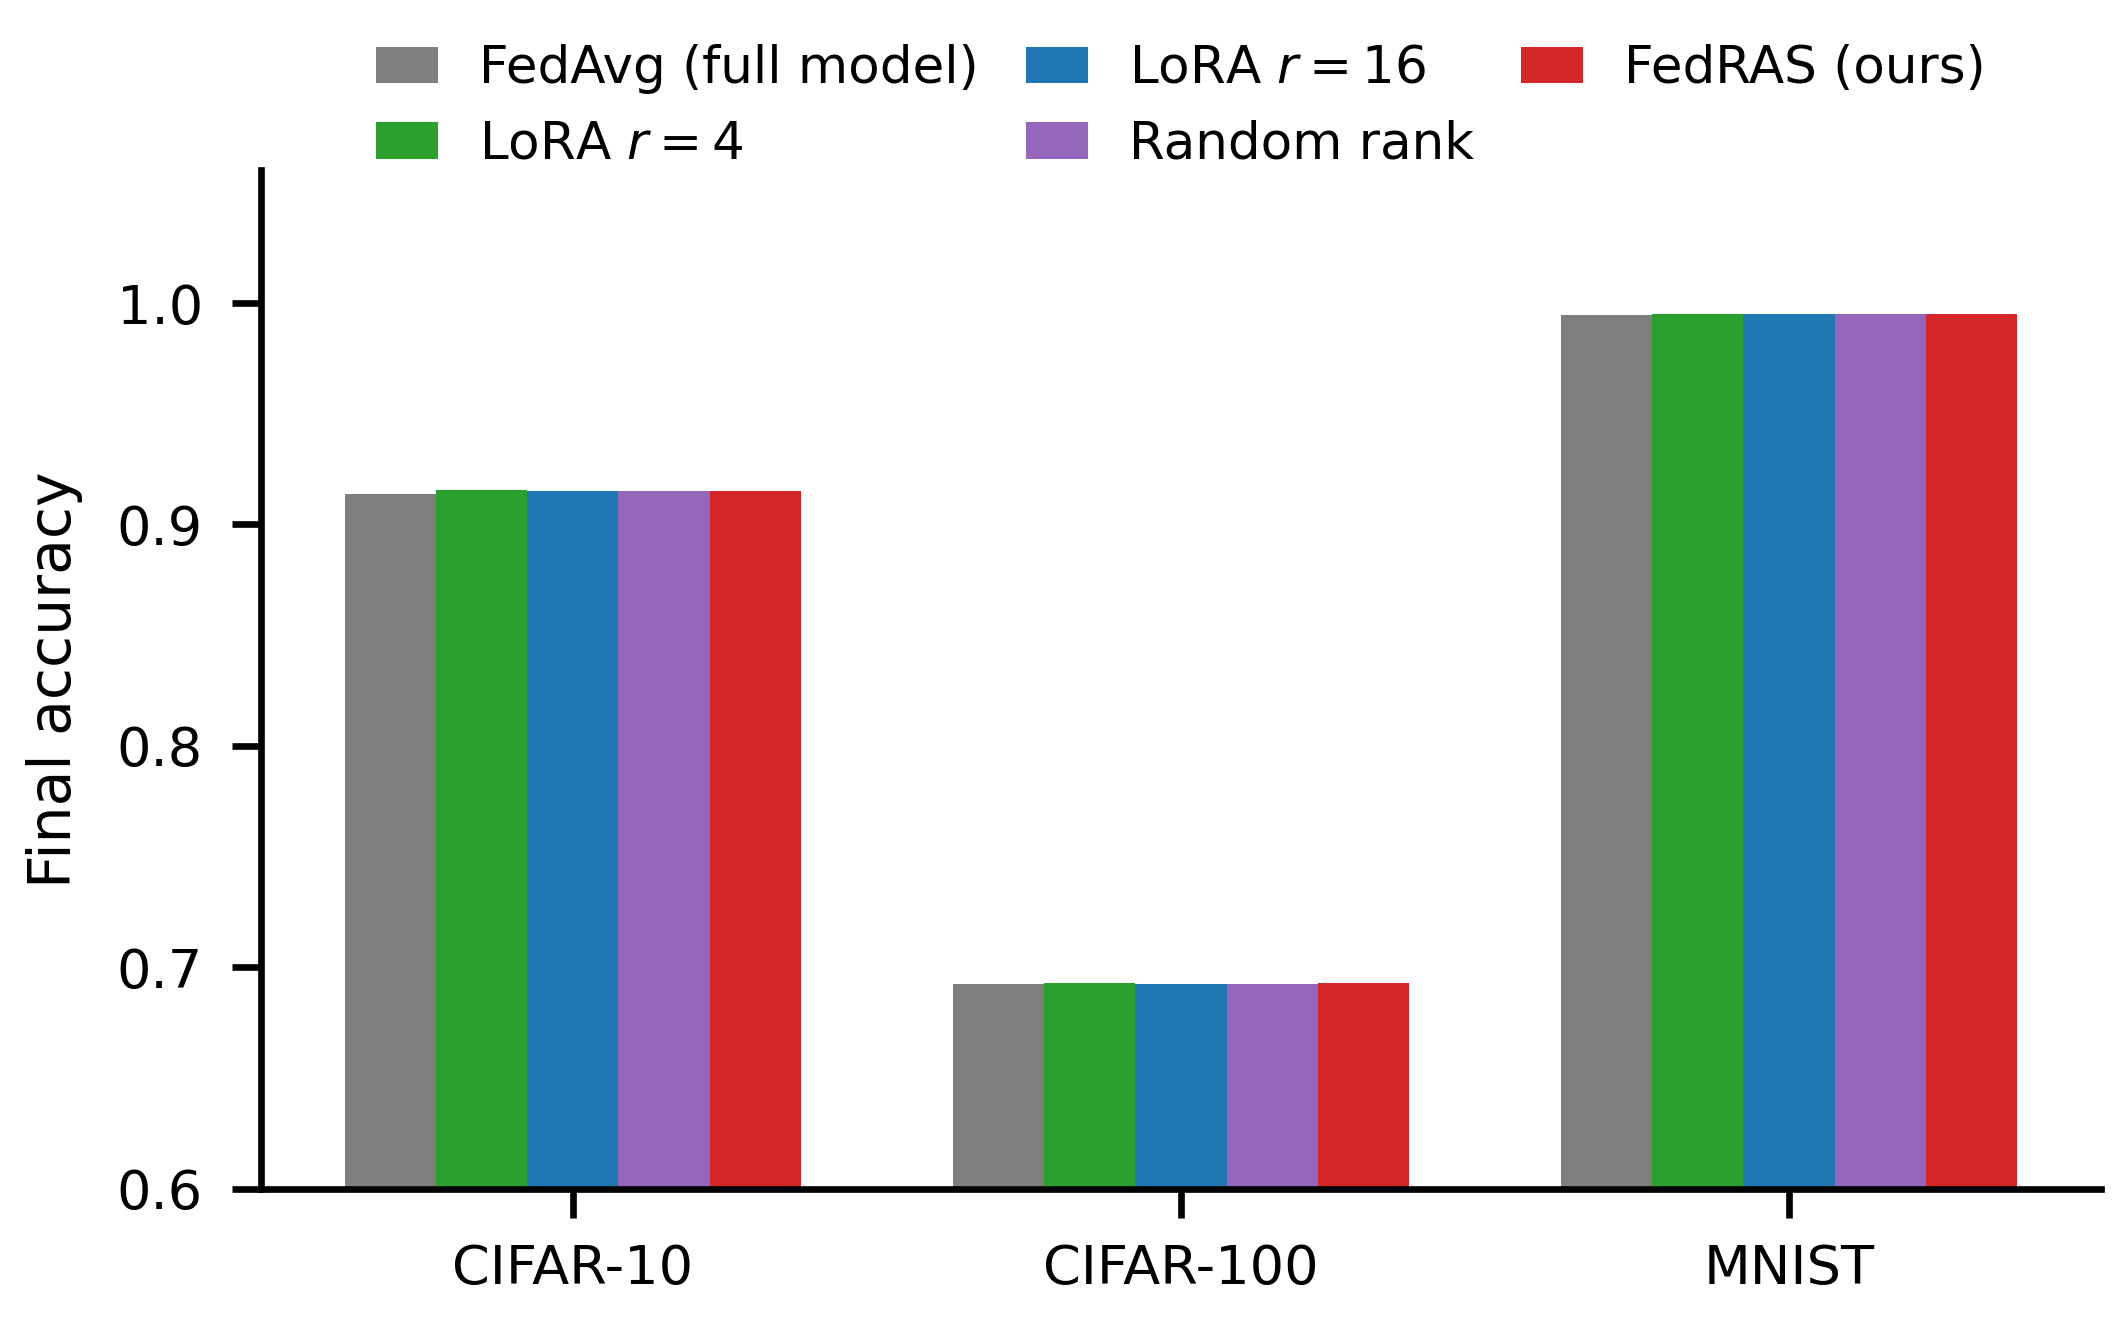
\includegraphics[width=0.8\columnwidth]{recolored_figures/fig_cross_dataset.png}
%DIFDELCMD < %%%
\DIFdelendFL \DIFaddbeginFL 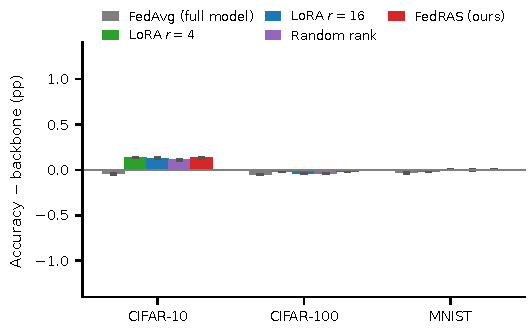
\includegraphics[width=0.8\columnwidth]{recolored_figures/fig_cross_dataset}
\DIFaddendFL \caption{Final accuracy across datasets\DIFdelbeginFL \DIFdelFL{under the nominal deadline (}\DIFdelendFL \DIFaddbeginFL \DIFaddFL{. CIFAR-10 uses ten seeds; CIFAR-100 and MNIST use }\DIFaddendFL five seeds\DIFdelbeginFL \DIFdelFL{)}\DIFdelendFL . The parity and equivalence findings of Table~\ref{tab:trainer} are not CIFAR-10-specific.}
\label{fig:crossds}
\end{figure}

\begin{table}[t]
\centering
\caption{Real trainer on non-IID CIFAR-10 at the nominal 2.0\,s deadline with \DIFdelbeginFL \DIFdelFL{five }\DIFdelendFL \DIFaddbeginFL \DIFaddFL{ten }\DIFaddendFL seeds. Accuracy is measured at round 40. Timely delivery ratio is timely deliveries divided by selected clients. Bytes per round is the sum of attempted uplink payloads for selected clients over rounds 30 to 39, at real serialized sizes. Mean rank is computed over delivered updates.}
\label{tab:trainer}
\resizebox{0.92\columnwidth}{!}{%
\begin{tabular}{lcccc}
\toprule
Method & Accuracy & Timely delivery ratio & MB/round & Mean rank\\
\midrule
FedAvg (full model) & $0.9135\pm0.0027$ & 0.17 & 52.86 & ---\\
FedLoRA $r{=}4$ & $0.9154\pm0.0016$ & 0.75 & 0.23 & 4.0\\
FedLoRA $r{=}16$ & $0.9153\pm0.0015$ & 0.73 & 0.90 & 16.0\\
Random rank & $0.9151\pm0.0016$ & 0.76 & 0.42 & 7.3\\
FedRAS (ours) & $0.9153\pm0.0016$ & 0.73 & 0.90 & 16.0\\
\bottomrule
\end{tabular}%
}
\end{table}

\subsection{Accuracy parity and rank invariance in the trainer}
Table~\ref{tab:trainer} reports \DIFdelbegin \DIFdel{five-seed }\DIFdelend \DIFaddbegin \DIFadd{ten-seed }\DIFaddend means and standard deviations after 40 federated rounds on CIFAR-10. All LoRA methods hold the backbone accuracy within one standard deviation of 0.914, whether the rank is fixed at 4, fixed at 16, drawn at random, or selected by the rank rule. Full-parameter updates spend $58.7\times$ the bytes of a rank-16 update, and they lose roughly three quarters of their timely deliveries, 0.17 against 0.73, because their 5.29\,MB payloads rarely fit the round deadline. The cross-dataset results in Fig.~\ref{fig:crossds} agree at 0.693 on CIFAR-100 and 0.995 on MNIST. At the nominal deadline the rank rule selects rank 16 for every client of every round, so FedRAS coincides with fixed rank 16 \DIFdelbegin \DIFdel{exactly, in bytes , }\DIFdelend \DIFaddbegin \DIFadd{in bytes and }\DIFaddend timeliness, and \DIFdelbegin \DIFdel{accuracy}\DIFdelend \DIFaddbegin \DIFadd{in accuracy up to floating-point nondeterminism}\DIFaddend ; this identity, rather than a tuned advantage, is what the nominal regime is meant to show. Fig.~\ref{fig:trainer_acc} shows the corresponding trajectories, stable over the 40 rounds for every rank policy.

\begin{figure}[t]
\centering
\DIFdelbeginFL %DIFDELCMD < \includegraphics[width=0.8\columnwidth]{fig_trainer_nominal.png}
%DIFDELCMD < %%%
\DIFdelendFL \DIFaddbeginFL 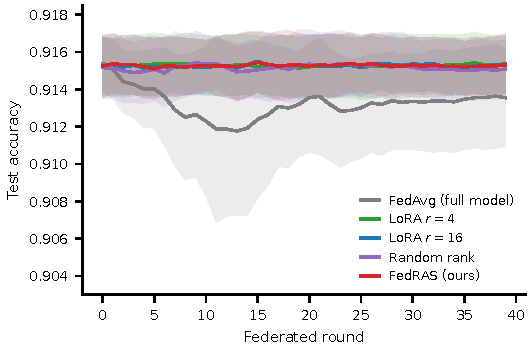
\includegraphics[width=0.8\columnwidth]{recolored_figures/fig_trainer_nominal}
\DIFaddendFL \caption{Real-trainer CIFAR-10 test accuracy over 40 federated rounds at the nominal deadline (mean over \DIFdelbeginFL \DIFdelFL{five }\DIFdelendFL \DIFaddbeginFL \DIFaddFL{ten }\DIFaddendFL seeds). All rank policies hold the pretrained-backbone accuracy; differences appear in bytes and timeliness, not accuracy.}
\label{fig:trainer_acc}
\end{figure}

\subsection{Deadline stress in the trainer}
Table~\ref{tab:stress} tightens the deadline to 0.1\,s and 0.05\,s\DIFdelbegin \DIFdel{with five seeds}\DIFdelend \DIFaddbegin \DIFadd{, with ten seeds at 0.1\,s and five seeds at 0.05\,s}\DIFaddend . Three effects emerge. First, FedRAS downshifts under pressure. Its delivered mean rank falls from 16.0 at the nominal deadline to 12.7 at 0.1\,s and 8.1 at 0.05\,s, where the delivery hazard \eqref{eq:hazard} makes rank-16 payloads marginal. Second, downshifting pays. At 0.1\,s, FedRAS delivers 0.49 timely updates against 0.41 for fixed rank 16 while transmitting 0.69\,MB against 0.90\,MB, i.e., 23\% fewer bytes; at 0.05\,s the gap widens to 0.49 against 0.27 timely deliveries at 51\% fewer bytes. Third, full-parameter updates collapse completely. Their timely delivery ratio is 0.00 at both stress deadlines, so not a single one of their 5.29\,MB updates arrives on time, and their bytes are attempted in vain at $58.7\times$ the cost.

\begin{table}[t]
\centering
\caption{Real trainer under deadline stress\DIFdelbeginFL \DIFdelFL{with five seeds}\DIFdelendFL . Accuracy is the round-40 mean and standard deviation. Timely delivery ratio, bytes per round, and mean delivered rank are averaged over rounds 30 to 39 at real serialized sizes. \DIFaddbeginFL \DIFaddFL{The 0.1\,s columns use ten seeds; the 0.05\,s columns use five seeds.}\DIFaddendFL }
\label{tab:stress}
\resizebox{0.92\columnwidth}{!}{%
\begin{tabular}{l cccc cccc}
\toprule
& \multicolumn{4}{c}{deadline 0.1\,s} & \multicolumn{4}{c}{deadline 0.05\,s}\\
\cmidrule(lr){2-5}\cmidrule(lr){6-9}
Method & Acc. & Timely & MB & Rank & Acc. & Timely & MB & Rank\\
\midrule
FedAvg (full model) & $0.9153\pm.0015$ & 0.00 & 52.86 & --- & $0.9147\pm.0016$ & 0.00 & 52.86 & ---\\
FedLoRA $r{=}4$ & $0.9154\pm.0016$ & 0.62 & 0.23 & 4 & $0.9144\pm.0015$ & 0.57 & 0.23 & 4\\
FedLoRA $r{=}16$ & $0.9149\pm.0019$ & 0.41 & 0.90 & 16 & $0.9143\pm.0020$ & 0.27 & 0.90 & 16\\
Random rank & $0.9153\pm.0017$ & 0.56 & 0.42 & 6.2 & $0.9143\pm.0015$ & 0.46 & 0.42 & 5.7\\
FedRAS (ours) & $0.9154\pm.0018$ & 0.49 & 0.69 & 12.7 & $0.9143\pm.0014$ & 0.49 & 0.44 & 8.1\\
\bottomrule
\end{tabular}%
}
\end{table}

Accuracy spreads remain within about two standard deviations, which is consistent with the parity claim. The scheduling metrics are where the methods separate. Fig.~\ref{fig:trainer_dl} shows the \DIFdelbegin \DIFdel{five-}\DIFdelend \DIFaddbegin \DIFadd{ten-}\DIFaddend seed stress trajectories, and Fig.~\ref{fig:rankdyn} visualizes the mechanism directly: the delivered rank of FedRAS holds 16 under the nominal deadline, tracks 13 under the 0.1\,s deadline, and tracks 8 under the 0.05\,s deadline, whereas the annealed baseline follows its fixed heat--cool path regardless of link state. A ten-seed replication confirms these differences at conventional significance levels, with full statistics in Section~\ref{sec:summary}. Under the 0.1\,s deadline, FedRAS transmits 23\% fewer bytes than fixed $r{=}16$, with a seed-mean bootstrap 95\% confidence interval from $-26.6\%$ to $-20.6\%$ and a two-sided Wilcoxon $p$ of 0.002; it delivers a higher timely delivery ratio in ten of ten seed pairs, by 22\% on average ($p{=}0.002$); and its accuracy is statistically equivalent within the pre-registered $\pm0.5$ percentage-point margin (TOST $p{<}10^{-6}$).

\begin{figure}[t]
\centering
\DIFdelbeginFL %DIFDELCMD < 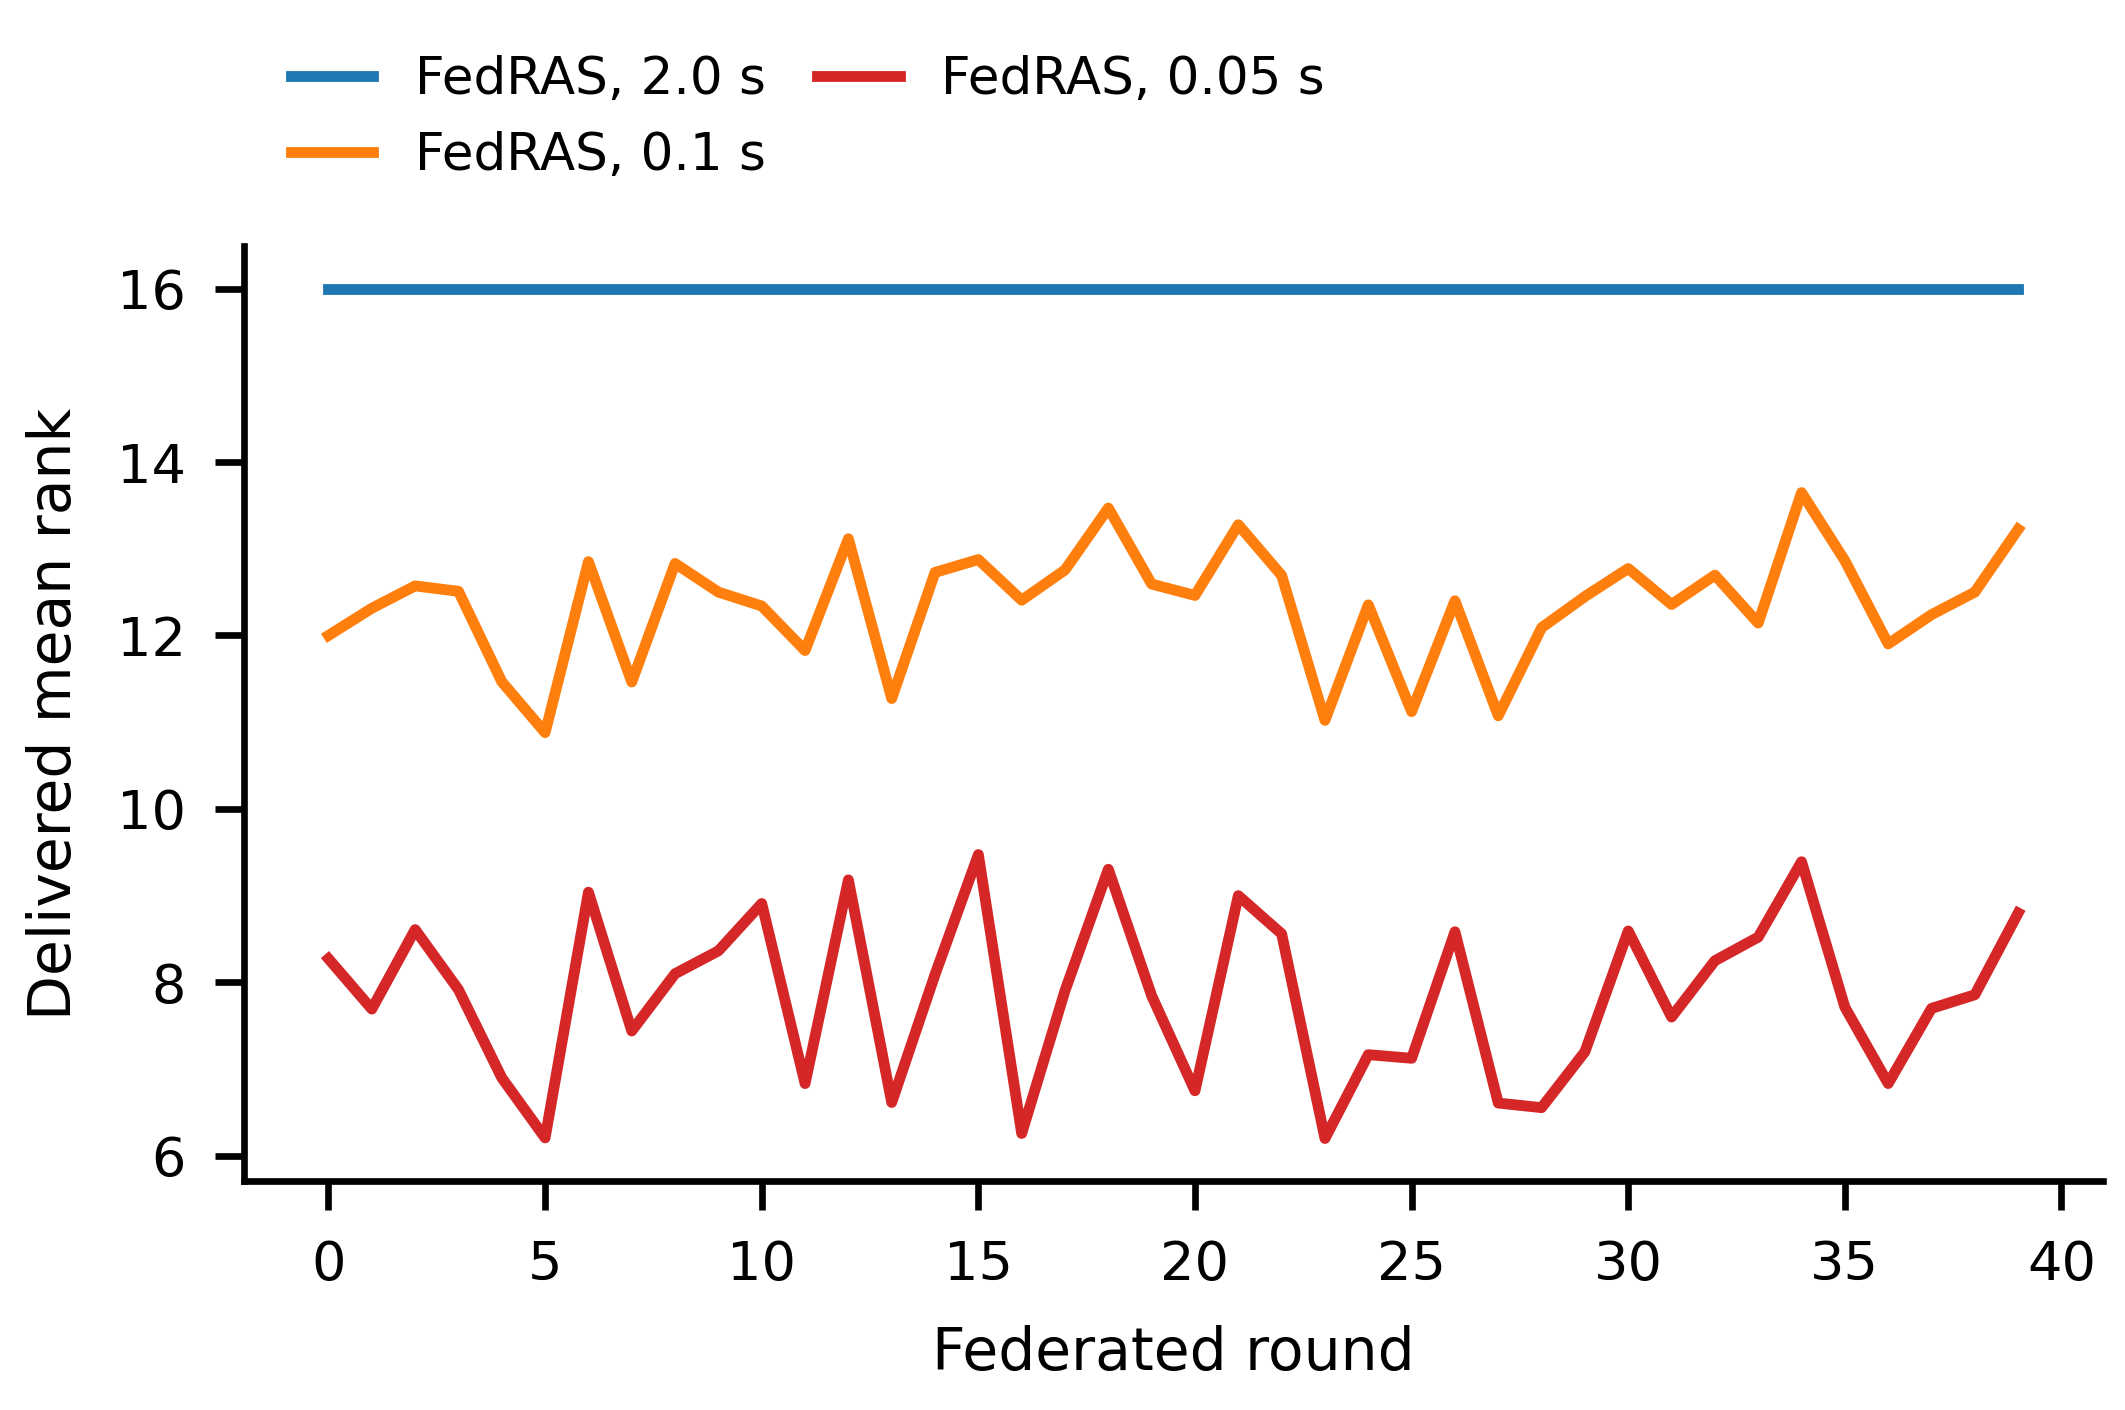
\includegraphics[width=0.8\columnwidth]{recolored_figures/fig_rank_dynamics.png}
%DIFDELCMD < %%%
\DIFdelendFL \DIFaddbeginFL 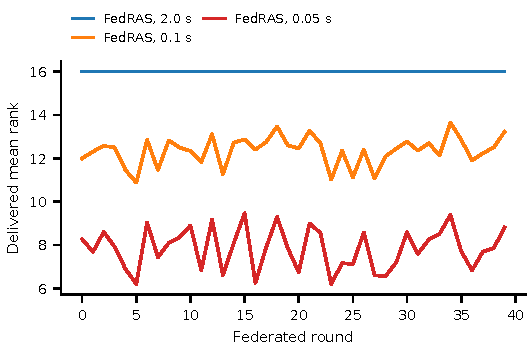
\includegraphics[width=0.8\columnwidth]{recolored_figures/fig_rank_dynamics}
\DIFaddendFL \caption{Delivered mean rank per round for FedRAS under three deadlines (\DIFaddbeginFL \DIFaddFL{ten seeds for 2.0 s and 0.1 s, }\DIFaddendFL five seeds \DIFaddbeginFL \DIFaddFL{for 0.05 s}\DIFaddendFL ), against the fixed annealing schedule of the SA-FedLoRA-style baseline at 0.1\,s. FedRAS is link-aware, holding high rank when possible and downshifting under pressure.}
\label{fig:rankdyn}
\end{figure}

\begin{figure}[t]
\centering
\DIFdelbeginFL %DIFDELCMD < \includegraphics[width=0.8\columnwidth]{fig_trainer_stress.png}
%DIFDELCMD < %%%
\DIFdelendFL \DIFaddbeginFL 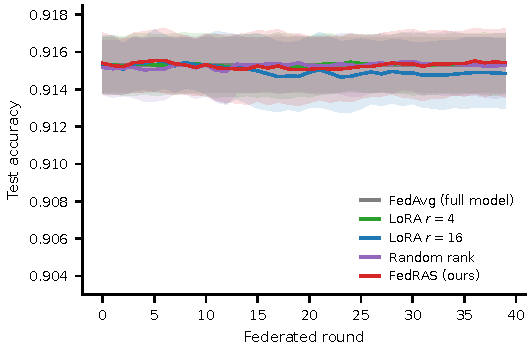
\includegraphics[width=0.8\columnwidth]{recolored_figures/fig_trainer_stress}
\DIFaddendFL \caption{Real-trainer accuracy trajectories under the 0.1\,s deadline (\DIFdelbeginFL \DIFdelFL{five }\DIFdelendFL \DIFaddbeginFL \DIFaddFL{mean over ten }\DIFaddendFL seeds). All methods remain stable; full-model updates deliver nothing and stay at the backbone.}
\label{fig:trainer_dl}
\end{figure}

\subsection{Broader stress matrix with mobility, heterogeneity, and cross-dataset checks}
Table~\ref{tab:extended} extends the study along further axes. A mobility-only scenario with Beta$(0.7,5)$ mobility at the nominal deadline leaves all LoRA policies at parity, so mobility alone does not force downshifting at this deadline. Extreme label heterogeneity with $\alpha{=}0.1$ reveals a second-order effect: rank-16 updates lose 0.32 percentage points relative to rank 4 (0.9107 versus 0.9139), consistent with capacity-amplified client drift, and full-parameter updates lose the most (0.9022). FedRAS follows the rank-16 trajectory here, so a heterogeneity-aware downshift is a natural extension. Loosening the deadline to 10\,s restores full-model timely delivery to 0.52 without changing any LoRA accuracy. Repeating the 0.1\,s deadline on CIFAR-100 and MNIST reproduces the CIFAR-10 stress picture. The scheduling conclusions are therefore not dataset-specific.

\begin{table}[t]
\centering
\caption{Extended stress matrix. Results use five seeds and report round-40 accuracy as mean over seeds. The mobility-only and $\alpha{=}1.0$ scenarios probe extreme conditions; the last two columns repeat the 0.1\,s deadline on CIFAR-100 and MNIST.}
\label{tab:extended}
\resizebox{0.92\columnwidth}{!}{%
\begin{tabular}{l ccccc}
\toprule
Scenario & FedAvg & $r{=}4$ & $r{=}16$ & Random & FedRAS\\
\midrule
deadline 10\,s & 0.9134 & 0.9144 & 0.9145 & 0.9141 & 0.9143\\
mobility 0.7 & 0.9115 & 0.9143 & 0.9141 & 0.9145 & 0.9141\\
$\alpha{=}0.1$ & 0.9022 & 0.9139 & 0.9107 & 0.9130 & 0.9109\\
$\alpha{=}1.0$ & 0.9142 & 0.9143 & 0.9144 & 0.9141 & 0.9144\\
CIFAR-100, 2.0\,s & 0.6925 & 0.6928 & 0.6926 & 0.6926 & 0.6929\\
CIFAR-100, 0.1\,s & 0.6927 & 0.6927 & 0.6929 & 0.6927 & 0.6928\\
MNIST, 2.0\,s & 0.9947 & 0.9949 & 0.9951 & 0.9950 & 0.9951\\
MNIST, 0.1\,s & 0.9947 & 0.9949 & 0.9950 & 0.9949 & 0.9950\\
\bottomrule
\end{tabular}%
}
\end{table}

\subsection{External baselines}
Table~\ref{tab:ext} adds three external baselines to the trainer. The first is an SA-FedLoRA-style schedule that heats the rank from 2 to 16 and cools it down over the 40 rounds, oblivious to link state \cite{yang2024safedlora}. The second is an Oort-style selector that samples $2K$ candidates and admits the top-$K$ by a data-size-and-recency utility at fixed rank \cite{oort2021oort}. The third is joint A/B training with plain averaging, the aggregation-level competitor of Section~\ref{sec:aggregation} \cite{guo2025fedsalora}.

\begin{table}[t]
\centering
\caption{External baselines in the real trainer on non-IID CIFAR-10 with \DIFdelbeginFL \DIFdelFL{five }\DIFdelendFL \DIFaddbeginFL \DIFaddFL{ten }\DIFaddendFL seeds. Accuracy is measured at round 40. Timely delivery ratio, bytes, and delivered mean rank are averaged over rounds 30--39.}
\label{tab:ext}
\resizebox{\columnwidth}{!}{%
\begin{tabular}{l cccc cccc}
\toprule
& \multicolumn{4}{c}{nominal deadline} & \multicolumn{4}{c}{deadline 0.1\,s}\\
\cmidrule(lr){2-5}\cmidrule(lr){6-9}
Method & Acc. & Timely & MB & Rank & Acc. & Timely & MB & Rank\\
\midrule
SA-FedLoRA-style annealing & $0.9154\pm.0016$ & 0.75 & 0.29 & 5.1 & $0.9153\pm.0016$ & 0.62 & 0.29 & 5.0\\
Oort-style utility, fixed rank & $0.9150\pm.0020$ & 0.76 & 0.45 & 8.0 & $0.9149\pm.0019$ & 0.54 & 0.45 & 8.0\\
Joint A/B, plain averaging & $0.9152\pm.0016$ & 0.73 & 0.90 & 16 & $0.9148\pm.0019$ & 0.41 & 0.90 & 16\\
\midrule
FedLoRA $r{=}16$ & $0.9153\pm.0015$ & 0.73 & 0.90 & 16 & $0.9149\pm.0019$ & 0.41 & 0.90 & 16\\
FedRAS (ours) & $0.9153\pm.0016$ & 0.73 & 0.90 & 16.0 & $0.9154\pm.0018$ & 0.49 & 0.69 & 12.7\\
\bottomrule
\end{tabular}%
}
\end{table}

The link-oblivious annealing schedule settles at low rank and therefore buys timely delivery with only 0.29\,MB per round, but it cannot increase rank when links improve, and its capacity ceiling is rank 5. The Oort-style selector improves selection at fixed rank. Joint A/B training matches frozen-factor training at the adopted learning rate\DIFdelbegin \DIFdel{; its stability cost appears under }\DIFdelend \DIFaddbegin \DIFadd{, and the ablations find no stability separation at }\DIFaddend an elevated learning rate \DIFdelbegin \DIFdel{, as the ablations show}\DIFdelend \DIFaddbegin \DIFadd{either, so the case for the frozen factor rests on exactness and upload reduction rather than on an observed stability gap}\DIFaddend .

\subsection{Full grid scheduling, same-cohort scheduling, and fair cohort}
\label{sec:dpvfair}
The trainer results so far use fair-cohort scheduling: the server samples the fixed cohort of ten clients and assigns each candidate its locally optimal rank. To attribute the value of exact scheduling, we evaluate two additional arms\DIFaddbegin \DIFadd{, }\DIFaddend over ten seeds \DIFaddbegin \DIFadd{at the nominal deadline and five seeds under stress}\DIFaddend . The full grid arm solves the dynamic program of Section~\ref{sec:solver} over the entire 20-client population under the participation cap and a 1.0\,MB budget, which equals ten rank-16 grid costs, so the budget binds only through downshifting or skipping. The same-cohort arm draws the identical cohort as fair cohort and restricts the same dynamic program to those candidates, isolating in-cohort rank allocation from candidate-pool widening.

\begin{table}[t]
\centering
\caption{Scheduling arms in the real trainer. Top: nominal 2.0\,s deadline over ten seeds. Bottom: 0.1\,s deadline over five seeds. Both arms of each comparison share the candidate protocol described in the text.}
\label{tab:dpvfair}
\DIFdelbeginFL %DIFDELCMD < \resizebox{\columnwidth}{!}{%
%DIFDELCMD < \begin{tabular}{l cccc}
%DIFDELCMD < \toprule
%DIFDELCMD < Method & Accuracy & Timely & MB & Rank\\
%DIFDELCMD < \midrule
%DIFDELCMD < \multicolumn{5}{l}{\emph{nominal 2.0\,s, ten seeds}}\\
%DIFDELCMD < Full DP (grid assignment, 1.0\,MB) & $0.9151\pm.0016$ & 0.82 & 0.90 & 16.0\\
%DIFDELCMD < Same-cohort DP (1.0\,MB) & $0.9152\pm.0018$ & 0.73 & 0.90 & 16.0\\
%DIFDELCMD < Fair cohort (FedRAS rule) & $0.9153\pm.0016$ & 0.73 & 0.90 & 16.0\\
%DIFDELCMD < FedLoRA $r{=}16$ & $0.9153\pm.0015$ & 0.73 & 0.90 & 16\\
%DIFDELCMD < \midrule
%DIFDELCMD < \multicolumn{5}{l}{\emph{stress 0.1\,s, five seeds}}\\
%DIFDELCMD < Full DP (grid assignment, 1.0\,MB) & $0.9138\pm.0011$ & 0.55 & 0.87 & 15.4\\
%DIFDELCMD < Same-cohort DP (1.0\,MB) & $0.9139\pm.0014$ & 0.51 & 0.70 & 12.7\\
%DIFDELCMD < Fair cohort (FedRAS rule) & $0.9154\pm.0018$ & 0.49 & 0.69 & 12.7\\
%DIFDELCMD < \bottomrule
%DIFDELCMD < \end{tabular}%
%DIFDELCMD < }
%DIFDELCMD < %%%
\DIFdelendFL \DIFaddbeginFL \resizebox{\columnwidth}{!}{%
\begin{tabular}{l cccc}
\toprule
Method & Accuracy & Timely & MB & Rank\\
\midrule
\multicolumn{5}{l}{\emph{nominal 2.0\,s, ten seeds}}\\
Full DP (grid assignment, 1.0\,MB) & $0.9151\pm.0016$ & 0.82 & 0.90 & 16.0\\
Same-cohort DP (1.0\,MB) & $0.9152\pm.0019$ & 0.73 & 0.90 & 16.0\\
Fair cohort (FedRAS rule) & $0.9153\pm.0016$ & 0.73 & 0.90 & 16.0\\
FedLoRA $r{=}16$ & $0.9153\pm.0015$ & 0.73 & 0.90 & 16\\
\midrule
\multicolumn{5}{l}{\emph{stress 0.1\,s, five seeds}}\\
Full DP (grid assignment, 1.0\,MB) & $0.9138\pm.0011$ & 0.55 & 0.87 & 15.4\\
Same-cohort DP (1.0\,MB) & $0.9139\pm.0014$ & 0.51 & 0.70 & 12.7\\
Fair cohort (FedRAS rule) & $0.9144\pm.0018$ & 0.51 & 0.70 & 13.0\\
\bottomrule
\end{tabular}%
}
\DIFaddendFL \end{table}

Table~\ref{tab:dpvfair} yields a clean decomposition. At the nominal deadline, the same-cohort DP coincides exactly with the per-client argmax rule, as \DIFdelbegin \DIFdel{it must when the budget does not bind and utilities are separable}\DIFdelend \DIFaddbegin \DIFadd{Proposition~\ref{prop:cohort} predicts when the all-rank-16 profile fits the budget}\DIFaddend ; the entire $+9$ percentage-point timely-delivery gain of the full DP (0.82 against 0.73) comes from admission over the wider candidate pool. Under the 0.1\,s deadline the pattern persists: the in-cohort DP matches the argmax rule, while the full DP reaches 0.55 against \DIFdelbegin \DIFdel{0.49 }\DIFdelend \DIFaddbegin \DIFadd{0.51 }\DIFaddend timely deliveries at 0.87 against \DIFdelbegin \DIFdel{0.69}\DIFdelend \DIFaddbegin \DIFadd{0.70}\DIFaddend \,MB. Exactness therefore pays through admission control over a heterogeneous pool, not through rank allocation inside a cohort, where the cheap per-client rule is already optimal \DIFaddbegin \DIFadd{(Proposition~\ref{prop:cohort})}\DIFaddend . This delimits when full grid scheduling is worth its coordination cost.

\subsection{Scheduler behavior at 500-client scale}
\label{sec:simsim}
Table~\ref{tab:sim} summarizes the simulator across regimes, with five seeds at the final round. The accuracy column is the bounded utility state of Section~\ref{sec:eval}, not a dataset accuracy. In the nominal regime, FedRAS matches fixed rank 16 at 0.914 and dominates every low-rank policy. Under the 0.1\,s deadline, FedRAS reaches 0.781 against 0.763 for fixed rank 16 at 21\% fewer bytes, and full-model updates deliver nothing. Under the binding 1.2\,MB budget, full-model updates cannot be admitted even once, while FedRAS and rank 16 tie at 0.797. The mobility-stress and 1000-client regimes show the same pattern. A final cell repeats the stylized protocol of the earlier literature: with the $s(r)$ payload model the ordering is preserved (FedRAS 0.413, rank 16 0.404, annealing 0.374), confirming that the conclusions are not an artifact of the payload accounting.

\begin{table}[t]
\centering
\caption{Scheduler simulation with 500 clients, 150 rounds, and five seeds. The accuracy column is a bounded scheduling proxy, not dataset accuracy. Timely delivery ratio is the mean delivery probability for admitted clients, and MB is the attempted uplink payload total for admitted clients in the final round. FedAvg refers to full-model updates at their real 5.29\,MB size.}
\label{tab:sim}
\DIFdelbeginFL %DIFDELCMD < \resizebox{0.98\columnwidth}{!}{%
%DIFDELCMD < \begin{tabular}{l ccc ccc ccc}
%DIFDELCMD < \toprule
%DIFDELCMD < & \multicolumn{3}{c}{Nominal 2.0\,s} & \multicolumn{3}{c}{Deadline 0.1\,s} & \multicolumn{3}{c}{Budget 1.2\,MB}\\
%DIFDELCMD < \cmidrule(lr){2-4}\cmidrule(lr){5-7}\cmidrule(lr){8-10}
%DIFDELCMD < Method & Acc. & Timely & MB & Acc. & Timely & MB & Acc. & Timely & MB\\
%DIFDELCMD < \midrule
%DIFDELCMD < FedAvg (full) & .310 & .35 & 26.5 & .093 & .00 & 26.5 & .093 & .00 & 0.0\\
%DIFDELCMD < $r{=}4$ & .744 & .75 & 0.8 & .689 & .64 & 0.8 & .744 & .75 & 0.8\\
%DIFDELCMD < $r{=}16$ & .914 & .73 & 2.5 & .763 & .42 & 2.5 & .797 & .76 & 1.2\\
%DIFDELCMD < Random & .816 & .75 & 1.3 & .709 & .57 & 1.3 & .803 & .75 & 1.2\\
%DIFDELCMD < Reliability-only & .635 & .76 & 0.5 & .606 & .70 & 0.5 & .635 & .76 & 0.5\\
%DIFDELCMD < SA-annealing & .842 & .76 & 0.5 & .730 & .70 & 0.5 & .796 & .76 & 0.5\\
%DIFDELCMD < FedRAS (ours) & .914 & .73 & 2.5 & \textbf{.781} & .50 & 2.0 & \textbf{.797} & .76 & 1.2\\
%DIFDELCMD < \bottomrule
%DIFDELCMD < \end{tabular}%
%DIFDELCMD < }
%DIFDELCMD < %%%
\DIFdelendFL \DIFaddbeginFL \resizebox{0.98\columnwidth}{!}{%
\begin{tabular}{l ccc ccc ccc}
\toprule
& \multicolumn{3}{c}{Nominal 2.0\,s} & \multicolumn{3}{c}{Deadline 0.1\,s} & \multicolumn{3}{c}{Budget 1.2\,MB}\\
\cmidrule(lr){2-4}\cmidrule(lr){5-7}\cmidrule(lr){8-10}
Method & Acc. & Timely & MB & Acc. & Timely & MB & Acc. & Timely & MB\\
\midrule
FedAvg (full) & .310 & .34 & 26.5 & .093 & .00 & 26.5 & .093 & .00 & 0.0\\
$r{=}4$ & .744 & .75 & 0.8 & .689 & .64 & 0.8 & .744 & .75 & 0.8\\
$r{=}16$ & .914 & .73 & 2.5 & .763 & .42 & 2.5 & .797 & .76 & 1.2\\
Random & .816 & .75 & 1.3 & .709 & .57 & 1.3 & .803 & .75 & 1.2\\
Reliability-only & .635 & .76 & 0.5 & .606 & .70 & 0.5 & .635 & .76 & 0.5\\
SA-annealing & .842 & .76 & 0.5 & .730 & .70 & 0.5 & .796 & .76 & 0.5\\
FedRAS (ours) & .914 & .73 & 2.5 & \textbf{.781} & .50 & 2.0 & \textbf{.797} & .76 & 1.2\\
\bottomrule
\end{tabular}%
}
\DIFaddendFL \end{table}

Fig.~\ref{fig:sim} shows the nominal and 0.1\,s trajectories, and Fig.~\ref{fig:simreg} the network-side view across regimes. Across the reported regimes, FedRAS is numerically best or tied for best; these simulator comparisons are descriptive unless an accompanying statistical test is reported.

\begin{figure}[t]
\centering
\DIFdelbeginFL %DIFDELCMD < 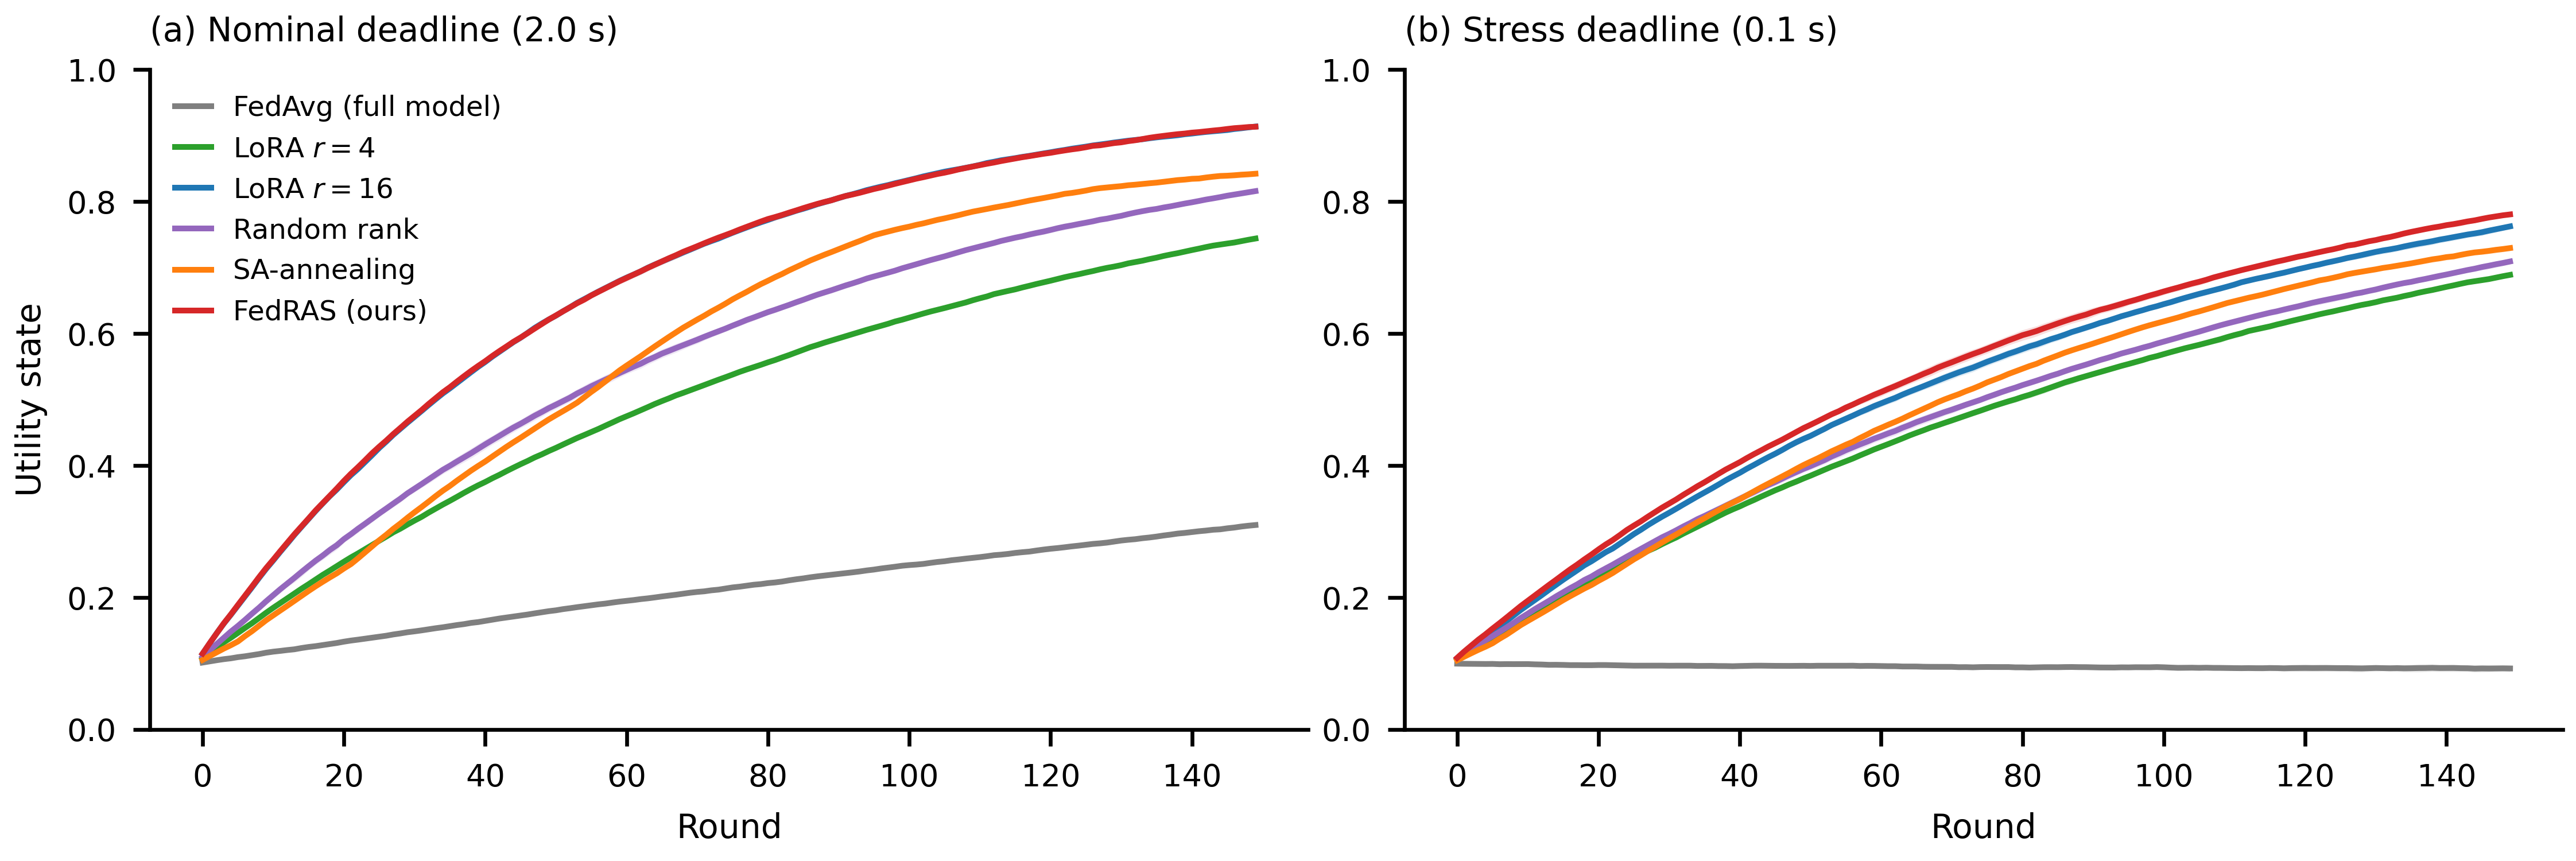
\includegraphics[width=0.98\columnwidth]{recolored_figures/fig_sim_accuracy.png}
%DIFDELCMD < %%%
\DIFdelendFL \DIFaddbeginFL 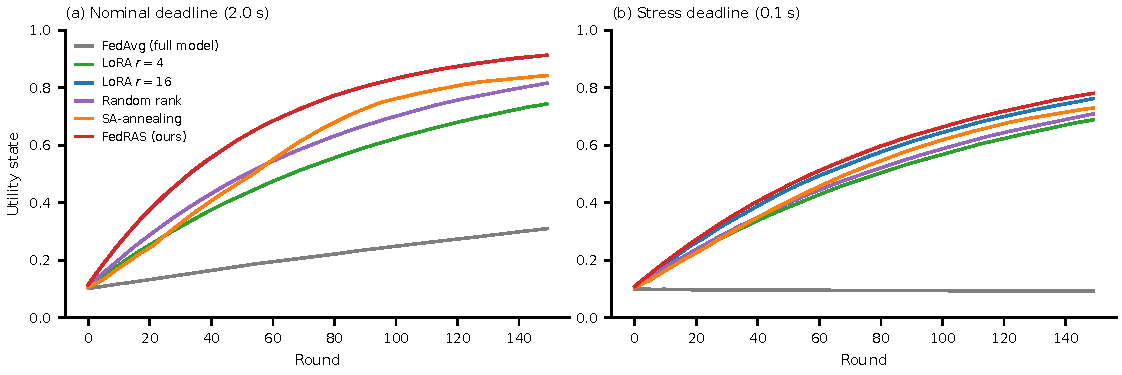
\includegraphics[width=0.98\columnwidth]{recolored_figures/fig_sim_accuracy}
\DIFaddendFL \caption{Scheduler simulation utility-state trajectories (mean over five seeds). \DIFdelbeginFL \DIFdelFL{Left: nominal }\DIFdelendFL \DIFaddbeginFL \DIFaddFL{(a)~Nominal }\DIFaddendFL 2.0\,s deadline, where FedRAS matches fixed rank 16. \DIFdelbeginFL \DIFdelFL{Right: }\DIFdelendFL \DIFaddbeginFL \DIFaddFL{(b)~}\DIFaddendFL 0.1\,s deadline, where FedRAS downshifting separates from fixed rank 16.}
\label{fig:sim}
\end{figure}

\begin{figure}[t]
\centering
\DIFdelbeginFL %DIFDELCMD < 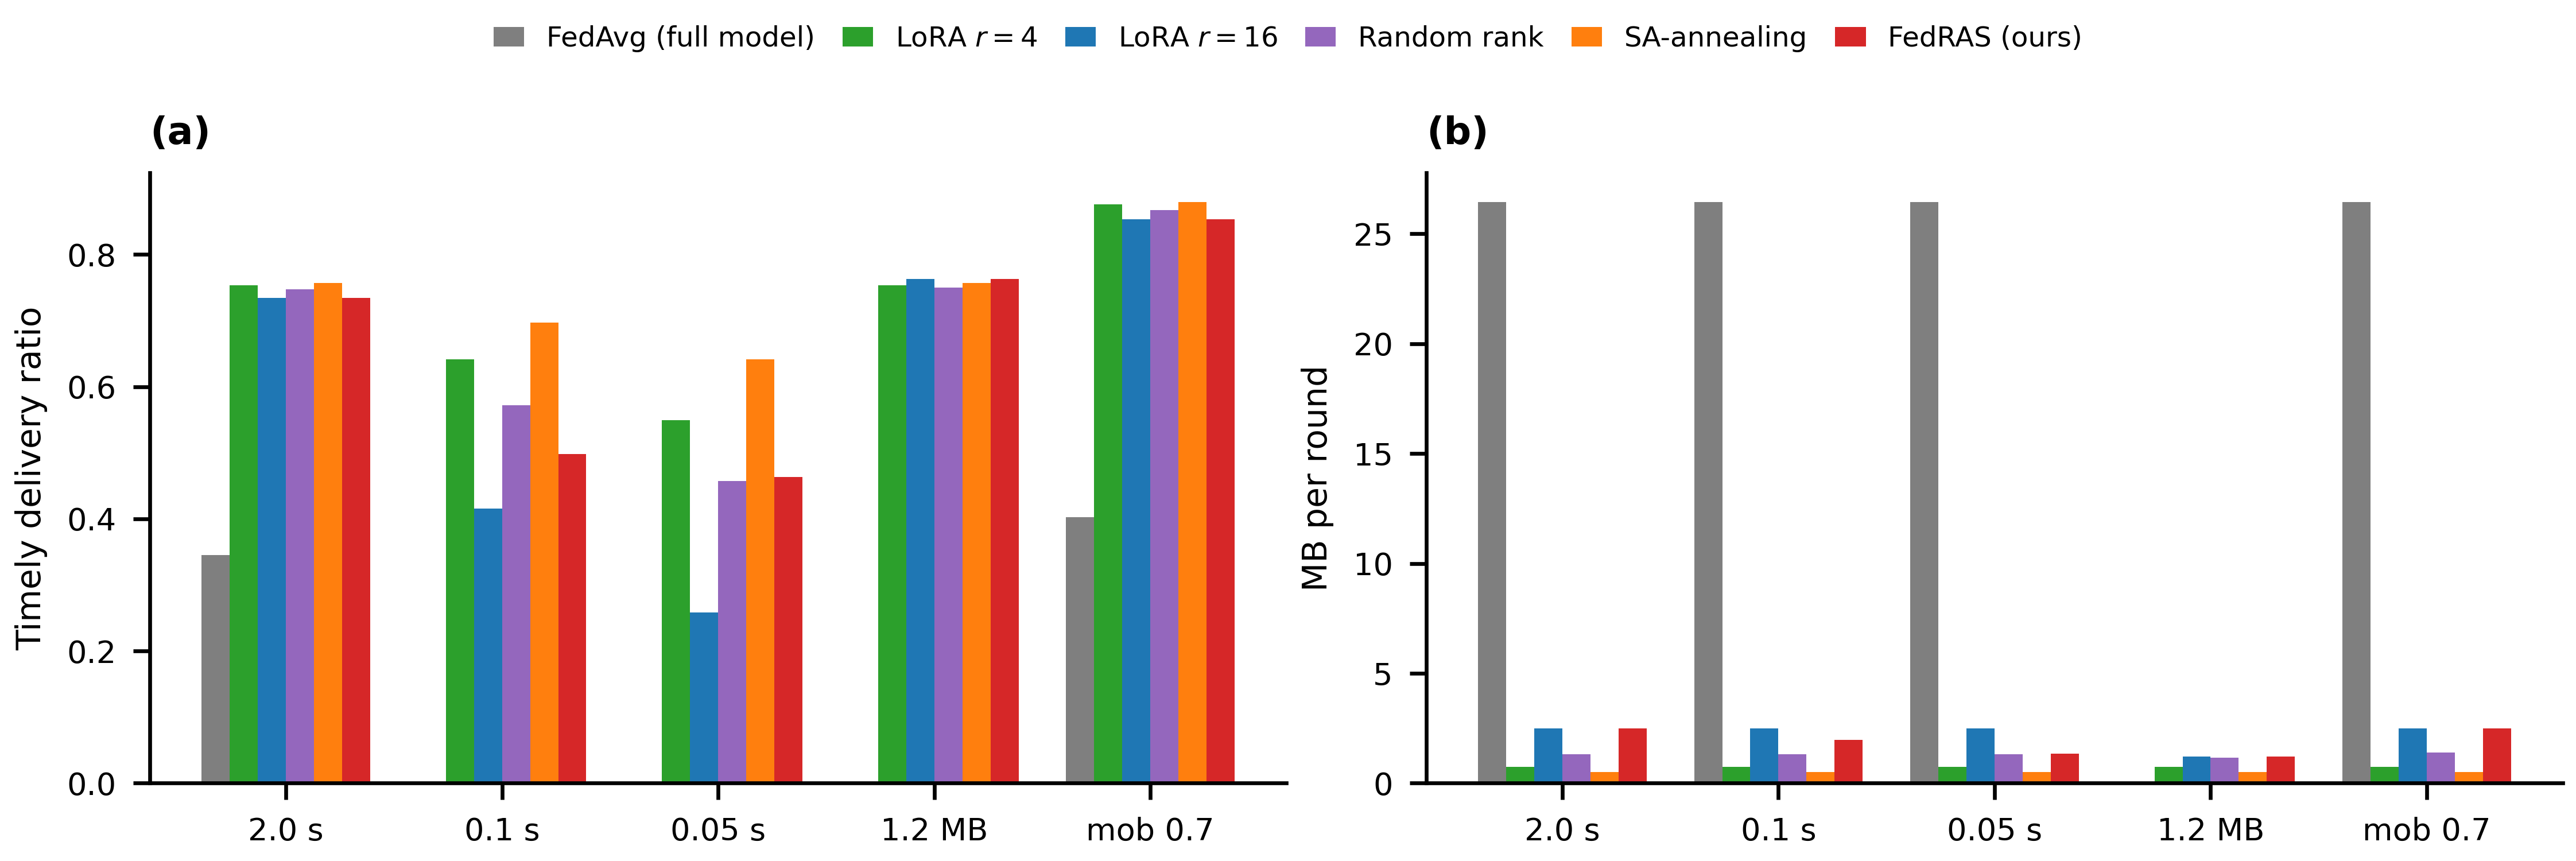
\includegraphics[width=0.98\columnwidth]{recolored_figures/fig_sim_regimes.png}
%DIFDELCMD < %%%
\DIFdelendFL \DIFaddbeginFL 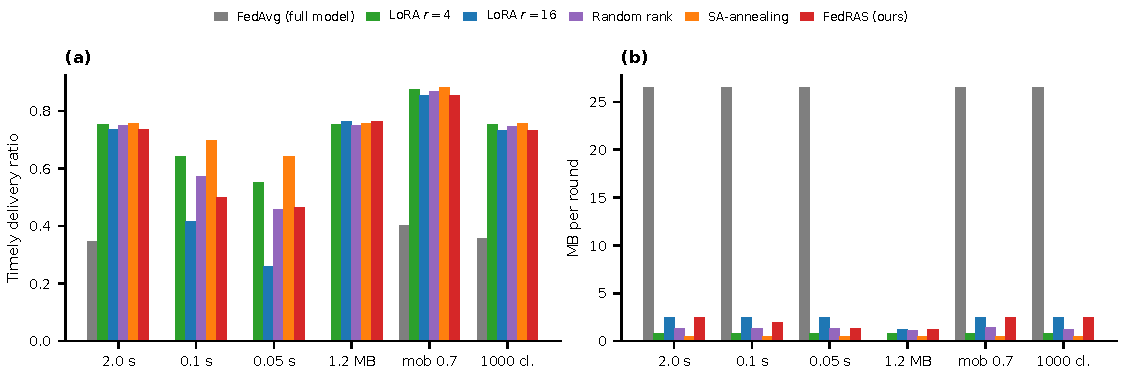
\includegraphics[width=0.98\columnwidth]{recolored_figures/fig_sim_regimes}
\DIFaddendFL \caption{Timely delivery ratio and attempted bytes per method across simulator regimes (five-seed means, final round). Full-model updates deliver nothing under stress and cannot be admitted at all under the binding budget.}
\label{fig:simreg}
\end{figure}

\subsection{Solver optimality and runtime}
\label{sec:dp_study}
Table~\ref{tab:dp} reports the scheduling study with the identical \DIFdelbegin \DIFdel{ceil }\DIFdelend \DIFaddbegin \DIFadd{ceiling }\DIFaddend discretization for the DP and every heuristic. When the byte budget is slack, value greedy is optimal and the fixed rank-16 rule is optimal whenever rank 16 is feasible for all cap clients, so the choice of scheduler matters little; the value-per-byte greedy, by contrast, collapses to a smallest-rank preference and loses up to 64\% of the objective. The interesting regimes are the binding ones. When the budget binds at 1.2\,MB, value-per-byte greedy loses 41 to 48\%, value greedy 28 to 36\%, and the cohort-myopic rule 48 to 55\%. The DP reaches the optimum of the discretized single-round estimated problem in every cell. Its runtime is 23 to 421\,ms for 500 clients depending on the budget-grid size, and it scales linearly to 1000 clients at 851\,ms, as Fig.~\ref{fig:dp} shows. This is compatible with per-round scheduling at minute-scale FL rounds.

A dedicated grid sweep with steps from 0.02 to 0.005\,MB compares each step against a 0.0025\,MB reference. In the binding 1.2\,MB regime the default 0.01\,MB step deviates by at most 3.1\%, and a 0.005\,MB step bounds the deviation to 2.4\%; slack regimes stay below 1\%. The grid exactness claim of Section~\ref{sec:solver} therefore applies to a grid whose quantization error is bounded, measured, and adjustable at a known runtime cost.

\DIFaddbegin \textbf{\DIFadd{Deployment recipe.}} \DIFadd{The results translate into three planning rules for a practitioner. Calibrate the deadline ladder from the real payload of the widest provisioned rank, so that the nominal deadline leaves rank $r_{\max}$ near-constraint-free while at least one stress deadline drives its timely delivery below one half. Size the byte budget at ten times the grid cost of rank $r_{\max}$, which forces the budget to bind only through downshifting or skipping. Finally, by Proposition~\ref{prop:cohort}, use the per-client argmax rule when the budget accommodates every candidate at rank $r_{\max}$ and invoke the full dynamic program only when the pool is heterogeneous enough that admission control matters.
}

\DIFaddend \begin{table}[t]
\centering
\caption{Solver study with 500 clients, $K{=}25$, and 30 instances per cell, all methods on the identical \DIFdelbeginFL \DIFdelFL{ceil }\DIFdelendFL \DIFaddbeginFL \DIFaddFL{ceiling }\DIFaddendFL grid. The table reports heuristic objective loss relative to the grid-based DP and DP runtime.}
\label{tab:dp}
\resizebox{\columnwidth}{!}{%
\begin{tabular}{cc cccc c}
\toprule
Deadline (s) & Budget (MB) & Greedy val/byte & Greedy value & Cohort myopic & Fixed $r{=}16$ & DP time (ms)\\
\midrule
2.0  & 30  & 63.6\% & 0.0\% & 40.9\% & 0.0\% & 421\\
2.0  & 4   & 63.6\% & 0.0\% & 40.9\% & 0.0\% & 51\\
2.0  & 1.2 & 47.8\% & 28.4\% & 48.9\% & 28.4\% & 23\\
1.0  & 30  & 62.7\% & 0.0\% & 40.0\% & 0.0\% & 415\\
1.0  & 4   & 62.7\% & 0.0\% & 43.0\% & 0.0\% & 51\\
1.0  & 1.2 & 47.3\% & 29.3\% & 48.3\% & 29.3\% & 23\\
0.1  & 30  & 52.8\% & 0.0\% & 51.9\% & 0.0\% & 415\\
0.1  & 4   & 52.6\% & 0.0\% & 52.0\% & 0.0\% & 51\\
0.1  & 1.2 & 41.0\% & 36.0\% & 54.8\% & 36.0\% & 23\\
\bottomrule
\end{tabular}%
}
\end{table}

\begin{figure}[t]
\centering
\DIFdelbeginFL %DIFDELCMD < 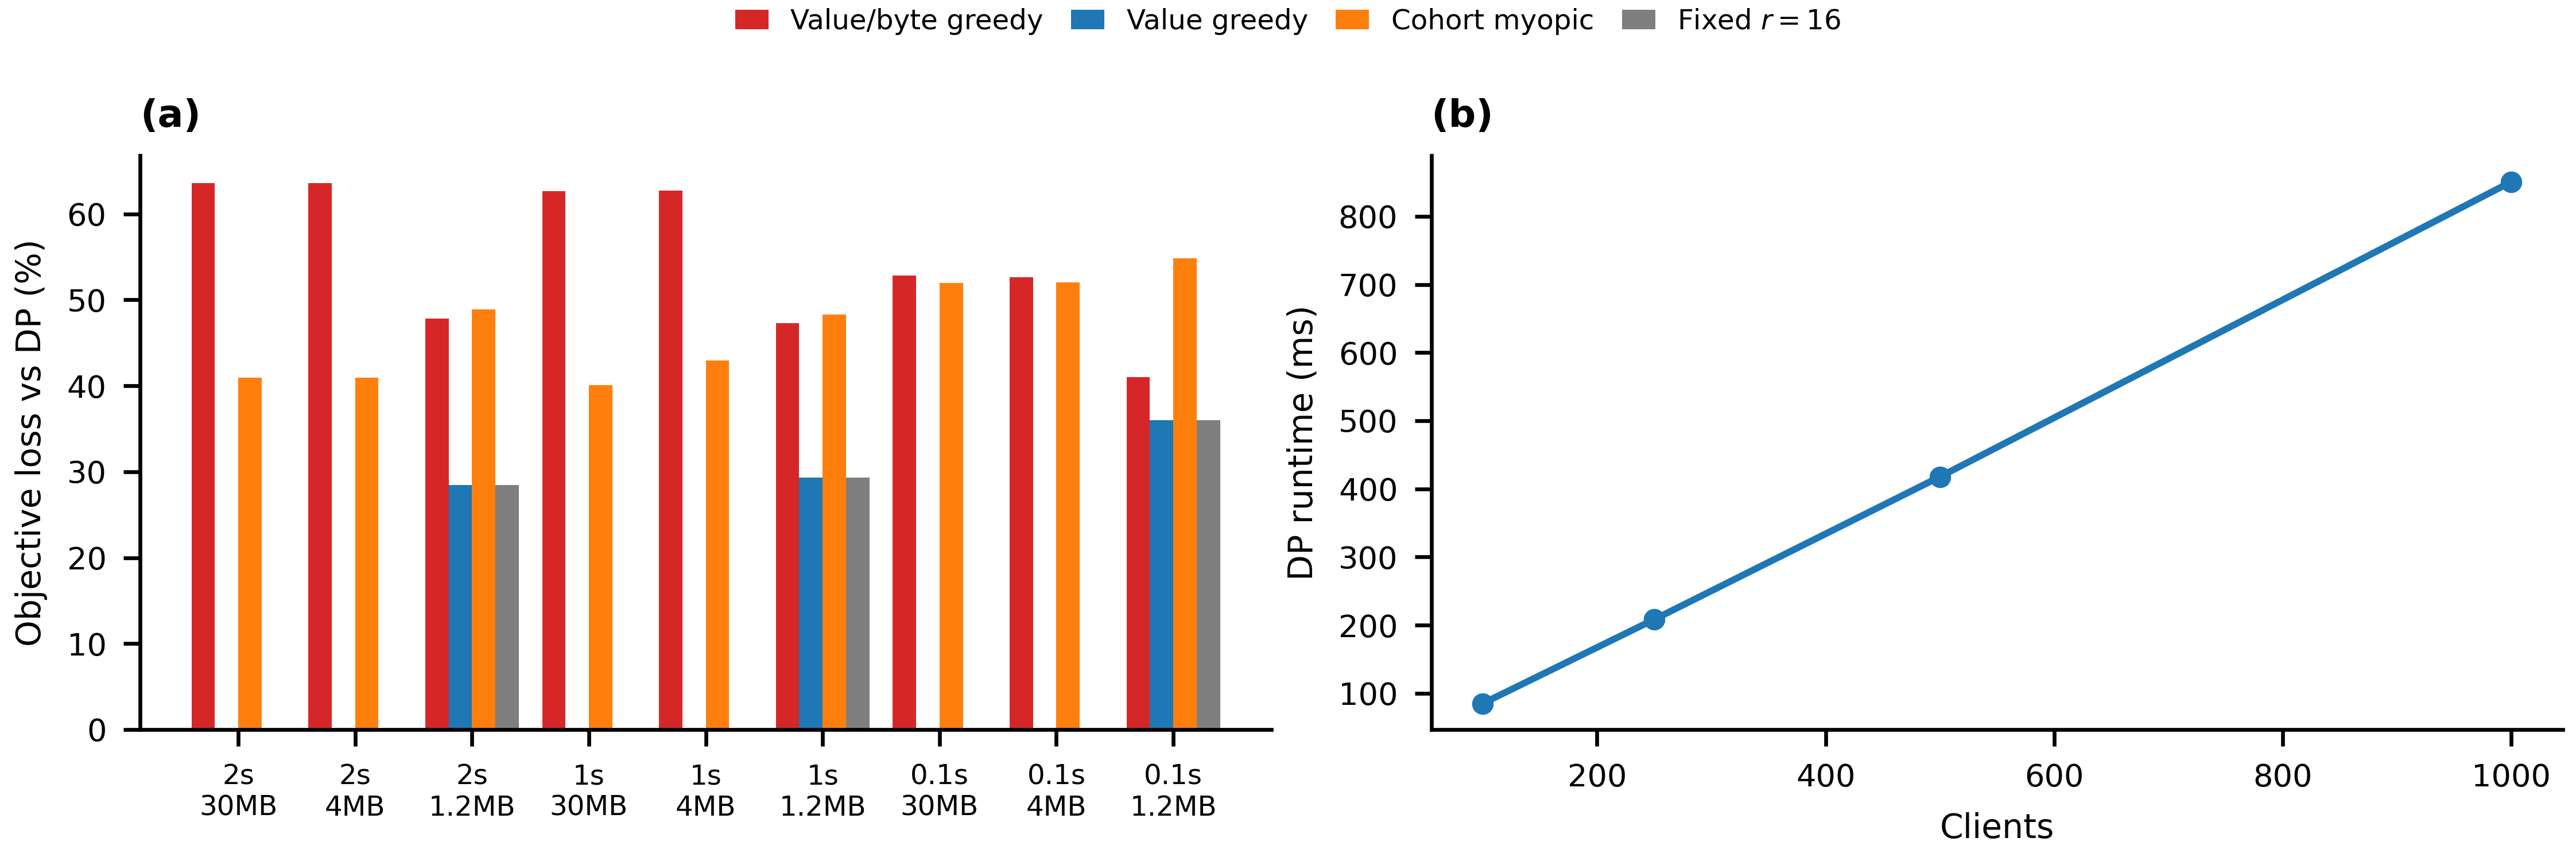
\includegraphics[width=0.98\columnwidth]{recolored_figures/fig_dp_study.png}
%DIFDELCMD < %%%
\DIFdelendFL \DIFaddbeginFL 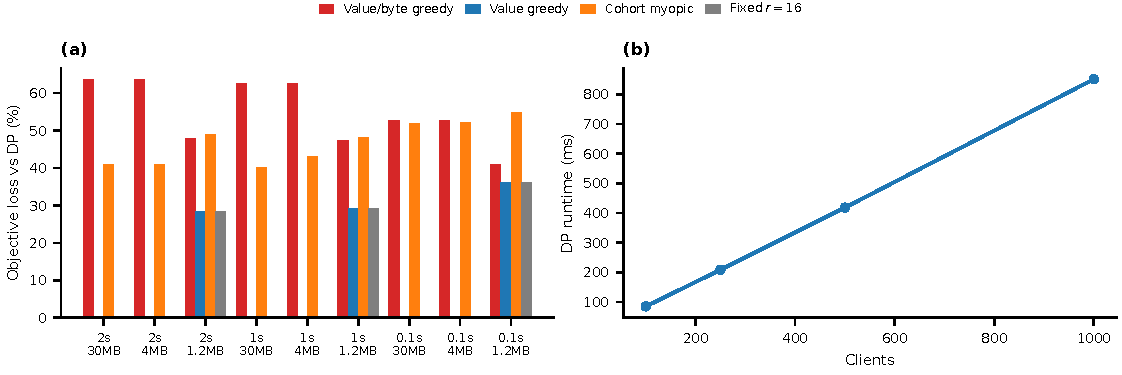
\includegraphics[width=0.98\columnwidth]{recolored_figures/fig_dp_study}
\DIFaddendFL \caption{Solver study. \DIFdelbeginFL \DIFdelFL{Left: objective }\DIFdelendFL \DIFaddbeginFL \DIFaddFL{(a)~Objective }\DIFaddendFL loss of the heuristics relative to the DP across deadline and budget cells. \DIFdelbeginFL \DIFdelFL{Right: }\DIFdelendFL \DIFaddbeginFL \DIFaddFL{(b)~}\DIFaddendFL DP runtime scaling with the client population.}
\label{fig:dp}
\end{figure}

\subsection{Sensitivity\DIFdelbegin \DIFdel{analysis}\DIFdelend \DIFaddbegin \DIFadd{, link profile, and predictor calibration}\DIFaddend }
\label{sec:sens}
Fig.~\ref{fig:sens} varies the provisioned adapter width, the cohort size, and the label heterogeneity of the trainer on CIFAR-10\DIFdelbegin \DIFdel{with five seeds}\DIFdelend \DIFaddbegin \DIFadd{. Each variant uses five seeds; the nominal reference column uses ten}\DIFaddend . Widening the adapter from $r_{\max}=8$ to 32 leaves accuracy flat while bytes rise from 0.45 to 1.80\,MB and timely delivery falls from 0.75 to 0.70; the provisioned width is a network-facing decision rather than an accuracy control. Cohort size from 5 to 20 leaves accuracy flat at linearly scaled bytes. Data heterogeneity from $\alpha=0.1$ to 1.0 moves accuracy as Table~\ref{tab:extended} shows at constant network cost. Per-decision scheduling cost is negligible in all settings: the per-client rank rule costs \DIFdelbegin \DIFdel{208}\DIFdelend \DIFaddbegin \DIFadd{about 0.1}\DIFaddend \,\DIFdelbegin \DIFdel{$\mu$s }\DIFdelend \DIFaddbegin \DIFadd{ms }\DIFaddend per decision, \DIFdelbegin \DIFdel{about 2}\DIFdelend \DIFaddbegin \DIFadd{roughly 1}\DIFaddend \,ms per round, against 23 to 421\,ms for the full grid-scheduling DP of Section~\ref{sec:dp_study}.

\textbf{SAGIN link profile.} Grouping the 20 clients into ground, aerial, and satellite classes with distinct rate and mobility laws reproduces the aggregate parity at the nominal deadline (accuracy 0.9141) while exposing the expected per-class structure: timely delivery is 0.71 for ground, 0.61 for aerial, and 0.49 for satellite clients. \DIFdelbegin \DIFdel{The rank rule downshifts within the constrained satellite class , and the aggregate byte bill is unchanged}\DIFdelend \DIFaddbegin \DIFadd{At this deadline the scheduler holds rank 16 across all classes, so the class gap reflects the link laws alone rather than rank allocation}\DIFaddend . This profile is a parameterized link model, not a measured trace; its role is to show that the scheduler responds sensibly to client-class heterogeneity, and calibration on measured traces remains open.

\textbf{Robustness to predictor error.} The calibration study of Fig.~\ref{fig:calib} doubles as a robustness probe. Injecting multiplicative lognormal noise with $\sigma=0.2$ into the predicted $\hat P_{\rm on}$ yields expected calibration error up to 0.078 while the assignment objective degrades by at most 0.95\%\DIFdelbegin \DIFdel{, and only in the tightest deadline and budget cell }\DIFdelend \DIFaddbegin \DIFadd{; no cell exceeds 1\%}\DIFaddend . Mis-prediction therefore costs optimality smoothly rather than catastrophically, and the observed delivery outcomes of Algorithm~\ref{alg:scheduler} are exactly the signal \DIFaddbegin \DIFadd{from which }\DIFaddend a calibrated predictor would re-fit.

\begin{figure}[t]
\centering
\DIFdelbeginFL %DIFDELCMD < 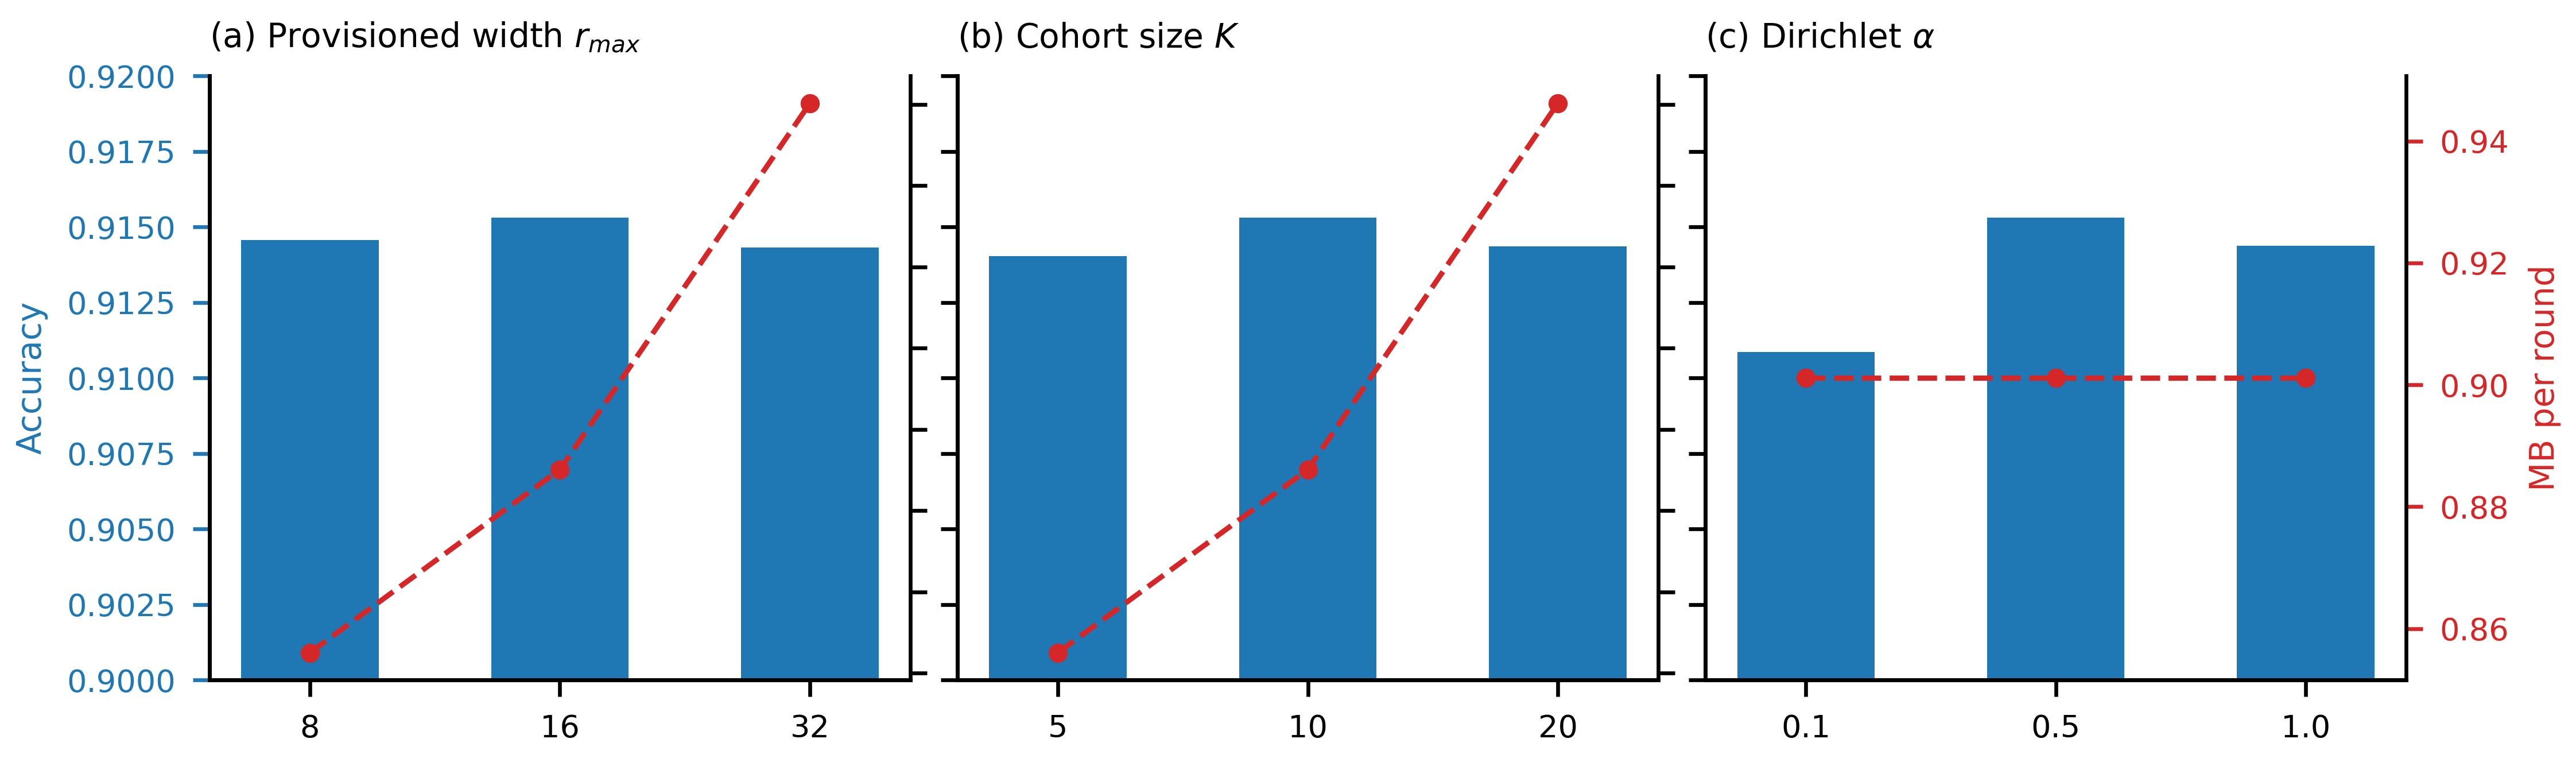
\includegraphics[width=0.98\columnwidth]{recolored_figures/fig_sensitivity.png}
%DIFDELCMD < %%%
\DIFdelendFL \DIFaddbeginFL 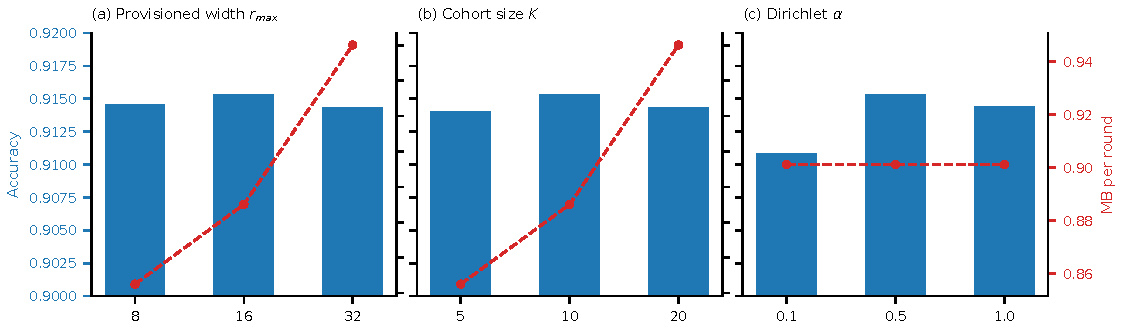
\includegraphics[width=0.98\columnwidth]{recolored_figures/fig_sensitivity}
\DIFaddendFL \caption{Sensitivity of the trainer to provisioned adapter width, cohort size, and label heterogeneity on CIFAR-10 with FedRAS (five seeds \DIFaddbeginFL \DIFaddFL{per variant; the nominal reference column uses ten seeds}\DIFaddendFL ). Accuracy is flat in $r_{\max}$, cohort size, and $\alpha$ across the tested ranges; their effect is on bytes and delivered updates (red, right axis).}
\label{fig:sens}
\end{figure}

\begin{figure}[t]
\centering
\DIFdelbeginFL %DIFDELCMD < 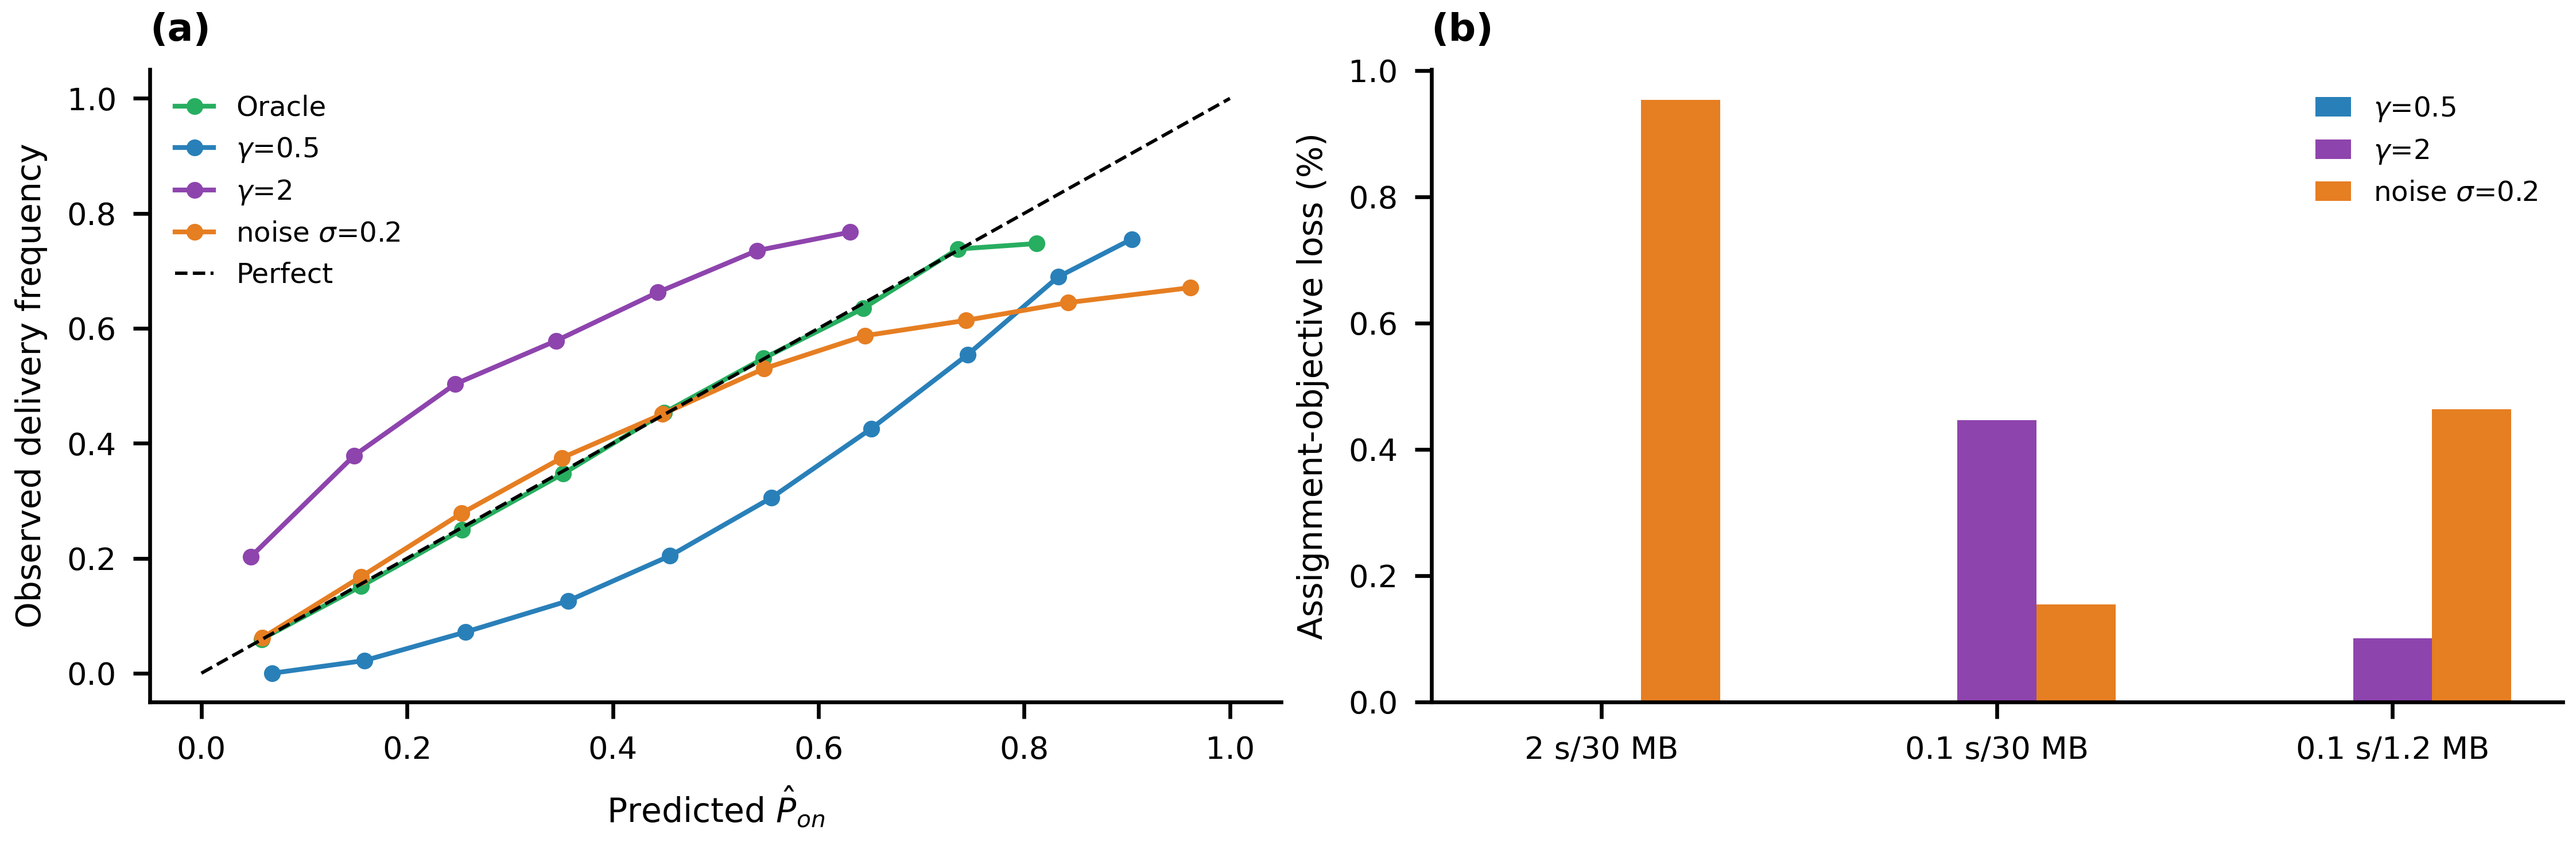
\includegraphics[width=0.8\columnwidth]{recolored_figures/fig_calibration.png}
%DIFDELCMD < %%%
\DIFdelendFL \DIFaddbeginFL 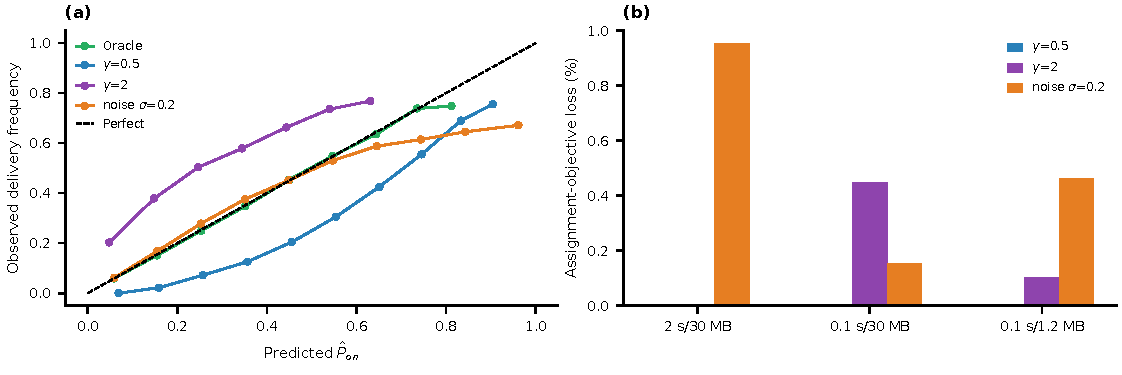
\includegraphics[width=0.8\columnwidth]{recolored_figures/fig_calibration}
\DIFaddendFL \caption{Delivery-predictor calibration study (500 clients, 150 round-instances per cell). The left panel shows reliability at the 0.1\,s deadline. With oracle link state the hazard-form predictor is calibrated by construction, while the power-distorted ($\gamma$) and noisy variants are measurably miscalibrated. The right panel shows the assignment-objective loss of optimizing against the distorted predictor, evaluated under true probabilities, at most 1\% \DIFdelbeginFL \DIFdelFL{and only }\DIFdelendFL in \DIFdelbeginFL \DIFdelFL{the tightest }\DIFdelendFL \DIFaddbeginFL \DIFaddFL{every }\DIFaddendFL cell.}
\label{fig:calib}
\end{figure}

\textbf{Calibration of the delivery predictor.} Calibration itself is measurable, and its scheduling cost is bounded, as Fig.~\ref{fig:calib} shows. On the link model of Section~\ref{sec:model}, the deployed predictor with oracle link state is calibrated by construction, with an expected calibration error of 0.003 to 0.004. Deliberately mis-calibrated variants $\hat P^{\gamma}$ with $\gamma$ of 0.5 and 2 reach an error up to 0.22. The resulting assignment-objective loss \DIFdelbegin \DIFdel{, however, stays at most 0.95\% and is confined to the tightest deadline and budget cell }\DIFdelend \DIFaddbegin \DIFadd{stays below 1\% in every cell. Its placement follows the structure of the predictor's error: the $\gamma$-distorted predictors cost more under the stress deadline (up to 0.45\%), where rank ordering matters most, while predictor noise costs the most in the nominal slack cell (0.95\%), where it distorts an otherwise near-uniform rank preference}\DIFaddend . Even sizeable miscalibration therefore leaves the rank ordering largely intact, and the observed outcomes expose \DIFdelbegin \DIFdel{it for }\DIFdelend \DIFaddbegin \DIFadd{the miscalibration and support }\DIFaddend per-client recalibration. Calibration on measured traces remains open and is taken up in Section~\ref{sec:discussion}.

\subsection{Component ablations}
Table~\ref{tab:ablation} reports component ablations at the nominal deadline. In the parity regime, no removal measurably changes final accuracy, which is consistent with the claim that accuracy is carried by the backbone and not by the scheduler. The components instead shape scheduling behavior and aggregation correctness. Removing the capacity term collapses FedRAS to the minimum rank, the degenerate delivery-only policy that the capacity term exists to prevent; its capacity cost is invisible at nominal deadlines but material in the simulator, where reliability-only optimization loses 28 points of utility against rank 16 (Table~\ref{tab:sim}). Removing server momentum is accuracy-neutral here. The rank mask itself is network-metric-neutral at fixed rank policy: with the random-rank rule at the 0.1\,s deadline, masked and unmasked aggregation give 0.9143 and 0.9145 final accuracy with identical byte and timeliness profiles. The mask is nonetheless what keeps heterogeneous-rank aggregation per-slice exact whenever ranks mix, as Proposition~\ref{prop:agg} states, and its absence dilutes high-rank coordinates under mixed-rank rounds.

Under the elevated learning rate of 0.02, the frozen-factor rule and joint A/B training are statistically indistinguishable, with final accuracies of 0.9130 and 0.9132 and transient minima of 0.913 and 0.912 across rounds and seeds. The stability separation between the two aggregation rules observed in our preliminary stylized-payload experiments does not survive the corrected implementation at this horizon, so the frozen-factor rule is justified by the exactness of Proposition~\ref{prop:agg} and by its single-factor uploads, not by an empirical stability margin at this scale.

\begin{table}[t]
\centering
\caption{Component ablations, real trainer (non-IID CIFAR-10, five seeds, nominal deadline). The Min.\ column is the minimum over rounds of the per-round seed-mean accuracy in the elevated-learning-rate stability check at learning rate 0.02.}
\label{tab:ablation}
\DIFdelbeginFL %DIFDELCMD < \resizebox{\columnwidth}{!}{%
%DIFDELCMD < \begin{tabular}{l cc}
%DIFDELCMD < \toprule
%DIFDELCMD < Configuration & Accuracy & Min.\\
%DIFDELCMD < \midrule
%DIFDELCMD < Full system (ours) & $0.9153\pm.0016$ & ---\\
%DIFDELCMD < \midrule
%DIFDELCMD < w/o capacity term & $0.9145\pm.0014$ & ---\\
%DIFDELCMD < w/o frozen $A$ (joint A/B) & $0.9144\pm.0015$ & ---\\
%DIFDELCMD < w/o rank mask (fixed random rank, 0.1\,s) & $0.9145\pm.0016$ & ---\\
%DIFDELCMD < w/o server momentum & $0.9143\pm.0013$ & ---\\
%DIFDELCMD < \midrule
%DIFDELCMD < frozen $A$, lr 0.02 & $0.9130\pm.0012$ & 0.913\\
%DIFDELCMD < joint A/B, lr 0.02 & $0.9132\pm.0012$ & 0.912\\
%DIFDELCMD < \bottomrule
%DIFDELCMD < \end{tabular}%
%DIFDELCMD < }
%DIFDELCMD < %%%
\DIFdelendFL \DIFaddbeginFL \resizebox{\columnwidth}{!}{%
\begin{tabular}{l cc}
\toprule
Configuration & Accuracy & Min.\\
\midrule
Full system (ours) & $0.9144\pm.0013$ & ---\\
\midrule
w/o capacity term & $0.9145\pm.0014$ & ---\\
w/o frozen $A$ (joint A/B) & $0.9144\pm.0015$ & ---\\
w/o rank mask (fixed random rank, 0.1\,s) & $0.9145\pm.0016$ & ---\\
w/o server momentum & $0.9143\pm.0013$ & ---\\
\midrule
frozen $A$, lr 0.02 & $0.9130\pm.0012$ & 0.913\\
joint A/B, lr 0.02 & $0.9132\pm.0012$ & 0.912\\
\bottomrule
\end{tabular}%
}
\DIFaddendFL \end{table}

\subsection{Summary of findings}
\label{sec:summary}
Across both tiers, rank choice does not measurably change accuracy for the frozen backbone and 40-round horizon, and every accuracy comparison against fixed rank 16 passes the pre-registered TOST equivalence test at the $\pm0.5$ percentage-point margin. The main differences are on the network side. Full-parameter updates cost $58.7\times$ the bytes of a rank-16 upload, miss $83\%$ of nominal deadlines and all stress deadlines, and \DIFdelbegin \DIFdel{degrade accuracy below }\DIFdelend \DIFaddbegin \DIFadd{fail to improve on }\DIFaddend the backbone when only sparse updates arrive; an offline control without delivery modeling \DIFdelbegin \DIFdel{shows that the full model trains }\DIFdelend \DIFaddbegin \DIFadd{trains close }\DIFaddend to the backbone level\DIFdelbegin \DIFdel{when delivery is not the constraint}\DIFdelend , separating learning capacity from delivery feasibility.

FedRAS behaves as designed, holding high ranks on healthy links and downshifting under pressure. Over ten seeds at the 0.1\,s deadline it transmits 23\% fewer bytes than fixed rank 16 (bootstrap 95\% CI $[-26.6\%, -20.6\%]$, Wilcoxon $p{=}0.002$, matched-pairs rank-biserial 1.0), delivers 22\% more timely updates ($p{=}0.002$), and is accuracy-equivalent. At the nominal deadline it reduces to fixed rank-16 behavior at zero cost. The exact dynamic program pays through admission over the wider candidate pool, $+9$ percentage points of timely delivery at the nominal deadline and \DIFdelbegin \DIFdel{$+12\%$ }\DIFdelend \DIFaddbegin \DIFadd{$+8\%$ }\DIFaddend under stress, while the per-client argmax rule is already optimal inside a cohort \DIFdelbegin \DIFdel{. Grid scheduling remains affordable at 23 to 421\,ms per round for 500 clients.
}%DIFDELCMD < 

%DIFDELCMD < %%%
\DIFdel{The statistical evidence rests }\DIFdelend \DIFaddbegin \DIFadd{(Proposition~\ref{prop:cohort}). These tests rest }\DIFaddend on ten-seed replications of the headline trainer regimes with common random numbers within each seed\DIFdelbegin \DIFdel{. The tests }\DIFdelend \DIFaddbegin \DIFadd{; they }\DIFaddend support the stated network-side comparisons and \DIFdelbegin \DIFdel{accuracy equivalence. They }\DIFdelend \DIFaddbegin \DIFadd{the accuracy equivalence, and they }\DIFaddend do not establish accuracy dominance.

\section{Discussion and limitations}
\label{sec:discussion}
\textbf{Scope of claims.} The trainer demonstrates parity and equivalence, not rank-dependent accuracy gains. With a strong frozen backbone and 40 adaptation rounds, transmitted rank does not measurably change test accuracy. Claims that low rank limits adaptation quality would require longer horizons, weaker backbones, or distribution-shifted clients. The simulator capacity model is a scheduling abstraction, and its accuracy is a bounded scheduling proxy rather than a measured dataset accuracy.

\textbf{Backbone pretraining.} The centralized pretraining stage is a documented premise inherited from parameter-efficient FL practice; the federated phase adapts but does not train the backbone. Where no server-side corpus exists, self-supervised or public-data pretraining would be needed, and the parity result should be re-verified.

\textbf{Estimator assumptions.} The hazard-form delivery model \eqref{eq:hazard} assumes the closed-form exponential realization, and the experiments supply generated link states as oracle estimates. Production deployments should calibrate $P_{\rm on}$ per client from observed outcomes, for example with isotonic or Platt scaling monitored by a Brier score, and the scheduler treats the predictor as a plug-in. Calibration on measured wireless traces remains open.

\textbf{Myopia.} The DP is exact for the estimated per-round problem, not for the multi-round stochastic control problem induced by budget carry-over and mobility correlation; a horizon-aware policy could shift admissions across rounds and is a natural extension.

\textbf{Security.} This work schedules communication and does not propose protection, so we make no privacy claim. Frozen-factor training incidentally reduces the dimensionality of transmitted gradients, which shrinks the gradient-inversion surface. Formal statements require differential-privacy accounting or secure aggregation, which compose orthogonally with rank scheduling \cite{bonawitz2017secureagg,wei2023pfl_dp}.

\DIFdelbegin \DIFdel{A further observation from the stress matrix is that under extreme heterogeneity of }\DIFdelend \DIFaddbegin \textbf{\DIFadd{When FedRAS does not help.}} \DIFadd{Three settings bound the method's value. First, when links are healthy and the budget accommodates every candidate at the provisioned width, FedRAS reduces exactly to fixed rank 16 (Proposition~\ref{prop:cohort}): the scheduling layer adds coordination cost and nothing else, so the simpler fixed-rank configuration is preferable. Second, under extreme label heterogeneity (}\DIFaddend $\alpha{=}0.1$\DIFaddbegin \DIFadd{)}\DIFaddend , higher ranks lose \DIFdelbegin \DIFdel{a small amount }\DIFdelend \DIFaddbegin \DIFadd{0.32 percentage points }\DIFaddend of accuracy relative to rank 4 \DIFdelbegin \DIFdel{, consistent with }\DIFdelend \DIFaddbegin \DIFadd{through }\DIFaddend capacity-amplified client drift\DIFdelbegin \DIFdel{. The }\DIFdelend \DIFaddbegin \DIFadd{, and FedRAS follows the rank-16 trajectory and inherits that loss; conditioning the }\DIFaddend capacity term $G(r)$ \DIFdelbegin \DIFdel{could be conditioned }\DIFdelend on measured heterogeneity \DIFdelbegin \DIFdel{to capture this effect, which we leave }\DIFdelend \DIFaddbegin \DIFadd{is left }\DIFaddend as future work. \DIFaddbegin \DIFadd{Third, under tight deadlines the weakest client class still delivers least (satellite 0.49 in the grouped profile), because downshifting protects delivery but cannot create link capacity. FedRAS is therefore worth its coordination cost when deadlines are tight relative to real payloads or when the byte budget binds; outside those regimes, fixed rank 16 is the identical and simpler choice.
}\DIFaddend 

\textbf{Generality.} The trainer validates adapters on convolutional and linear layers of a CNN at $r_{\max}{=}16$ with 20 \DIFdelbegin \DIFdel{to 1000 clientsand }\DIFdelend \DIFaddbegin \DIFadd{clients, and the simulator extends the population to 1000, both under }\DIFaddend synthetic link distributions. Extension to transformer backbones, measured rather than synthetic links, and larger rank sets may change the payload slope, capacity curve, and empirical conclusions. The formulation can be tested in those settings. The study does not measure energy, system overhead beyond scheduler runtime, or client fairness and therefore makes no claim about those properties.

\section{Conclusion}
\label{sec:conclusion}
This paper reframed Federated LoRA over mobile edge networks as a deadline-aware client--rank scheduling problem in which the LoRA rank is a network-visible resource accounted at its real serialized size. We derived a rank-conditioned delivery model, formulated the per-round assignment as a multiple-choice knapsack under budget and participation caps, solved the grid-discretized assignment with a pseudo-polynomial dynamic program, and stabilized heterogeneous-rank aggregation with frozen-factor rank-masked averaging in which only the trainable factor is ever transmitted.

Experiments with a real federated LoRA trainer and a 500-client scheduler simulation, with deadlines calibrated to real payloads, show that FedRAS preserves backbone accuracy up to a pre-registered equivalence margin, delivers 22\% more timely updates and 23\% fewer bytes than fixed rank 16 under ten-seed deadline stress, and exposes the complete collapse of full-parameter updates, which spend $58.7\times$ the bytes and deliver nothing on time under stress. The exact scheduler recovers \DIFdelbegin \DIFdel{up to 64}\DIFdelend \DIFaddbegin \DIFadd{28 to 55}\DIFaddend \% expected useful updates over greedy heuristics \DIFdelbegin \DIFdel{in binding regimes }\DIFdelend \DIFaddbegin \DIFadd{when the budget binds, up to 64\% over value-per-byte pricing, }\DIFaddend at sub-second cost, and its measurable value in the trainer comes from admission over the candidate pool rather than in-cohort rank allocation. Future work includes horizon-aware stochastic scheduling, calibrated per-client delivery predictors on measured traces, protection mechanisms composed with rank scheduling, and validation on transformer backbones.

\section*{Declaration of competing interest}
The authors declare that they have no known competing financial interests or personal relationships that could have appeared to influence the work reported in this paper.

\section*{Acknowledgements}
The authors thank the members of the Information Engineering University research group for many useful discussions and for hands-on assistance with the experimental implementation.

\section*{Funding}
This research did not receive any specific grant from funding agencies in the public, commercial, or not-for-profit sectors.

\section*{CRediT authorship contribution statement}
\textbf{Wenyu Ma:} Methodology, Software, Validation, Investigation, Writing -- original draft.
\textbf{Tao Hu:} Conceptualization, Formal analysis, Supervision, Writing -- review and editing.
\textbf{Xinlei Liu:} Data curation, Investigation, Visualization.
All authors approved the submitted version and accept responsibility for the work.

\section*{Data availability}
The reproducibility package accompanying this submission contains the complete source code (trainer, simulator, solver, and analysis scripts), per-run configuration files, per-seed result tables, and the raw training logs supporting every table and figure in this study; a permanent repository DOI will be supplied at publication.

\section*{Declaration of generative AI and AI-assisted technologies in the manuscript preparation process}
During the preparation of this work the authors used AI-assisted tools for language editing and formatting support. The authors reviewed and edited all generated material and take full responsibility for the content of the published article.

\bibliographystyle{elsarticle-num}
\bibliography{references}
\end{document}
